%!TEX root = these.tex

\chapter[Contexte/Besoin/Applications]{plif}
\minitoc
\label{chap1}
\cleardoublepage

	\section{Biologie structurale}
	\subsection{Protéines}
	Les protéines sont des macromolécules que l'on retrouve dans les cellules de tous les organismes vivants. Elles assurent un très grand nombre de fonctions cellulaires (structuration de la cellule, mouvements et divisions cellulaires, communication intercellulaire, transport, par exemple de dioxygène, défense immunitaire) et biochimiques (liaison et fixations de molécules, catalyse de réactions biochimiques, etc.) au sein des cellules et des tissus. Elles participent aussi au conditionnement de l'acide désoxyribonucléique (ADN) et ) la régulation de l'expression génétique. L'étude de leur fonctionnement donc est essentielle à la compréhension du vivant.
	
	\paragraph{}
	Concrètement, une protéine est un ensemble (éventuellement un singleton) de chaînes d'acides aminés, reliés par des liaisons peptidiques, c'est-à-dire des liaisons covalentes entre une fonction carboxyle (–C(O)OH) et une fonction amine (un composé organique dérivé de l'ammoniac dont au moins un atome d'hydrogène a été remplacé par un groupe carboné). Ces chaînes d'acides aminés sont également appelées chaînes polypeptidiques, ou simplement polypeptides.
	
    \begin{figure}[htb]
        \begin{subfigure}{.4\textwidth}
            \centering
            {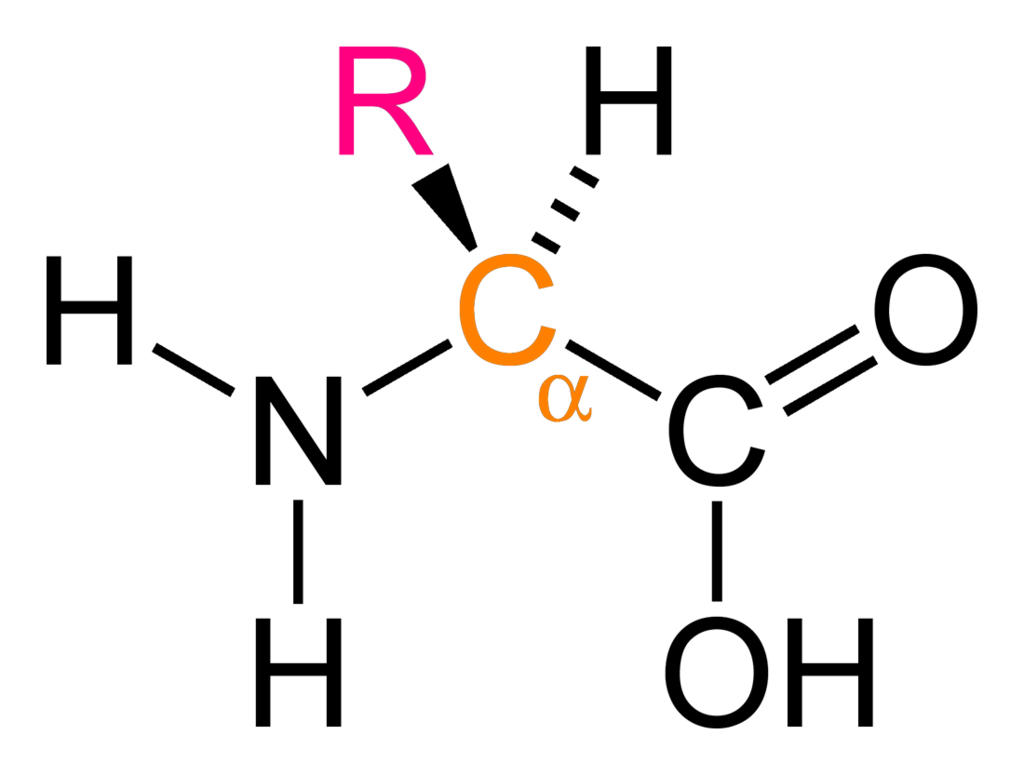
\includegraphics[height=4cm]{./figures/ch1/amino_acid_structure}}
            \caption{}
            \label{Fig:amino_acid_structure}
        \end{subfigure}
        \begin{subfigure}{.6\textwidth}
            \centering
            {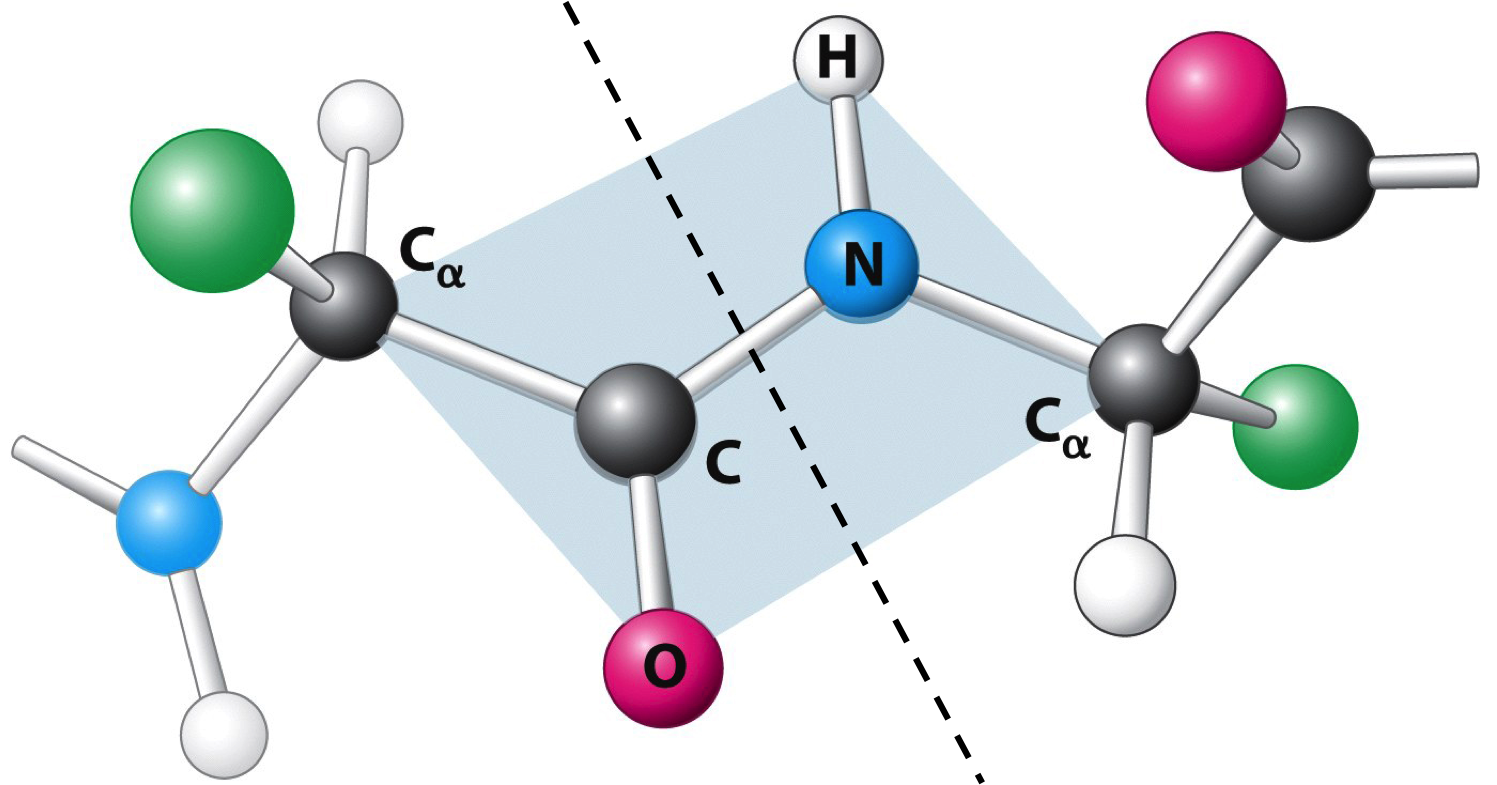
\includegraphics[height=4cm]{./figures/ch1/peptidic_bond.png}}
            \caption{}
            \label{Fig:peptide_bond}
        \end{subfigure}
        \caption{(a) Structure chimique d'un acide aminé. 
        (b) Illustration d'une liaison peptidique entre deux acides aminés (à gauche et à droite de la ligne pointillée). Cette liaison est une liaison covalente entre l'azote (N) de l'acide aminé de droite et le carbone (C) de l'acide aminé de gauche.  Source :~\cite{berg_biochemistry_2012}}
    \end{figure}
    
    \begin{figure}[ht]
		\centering
		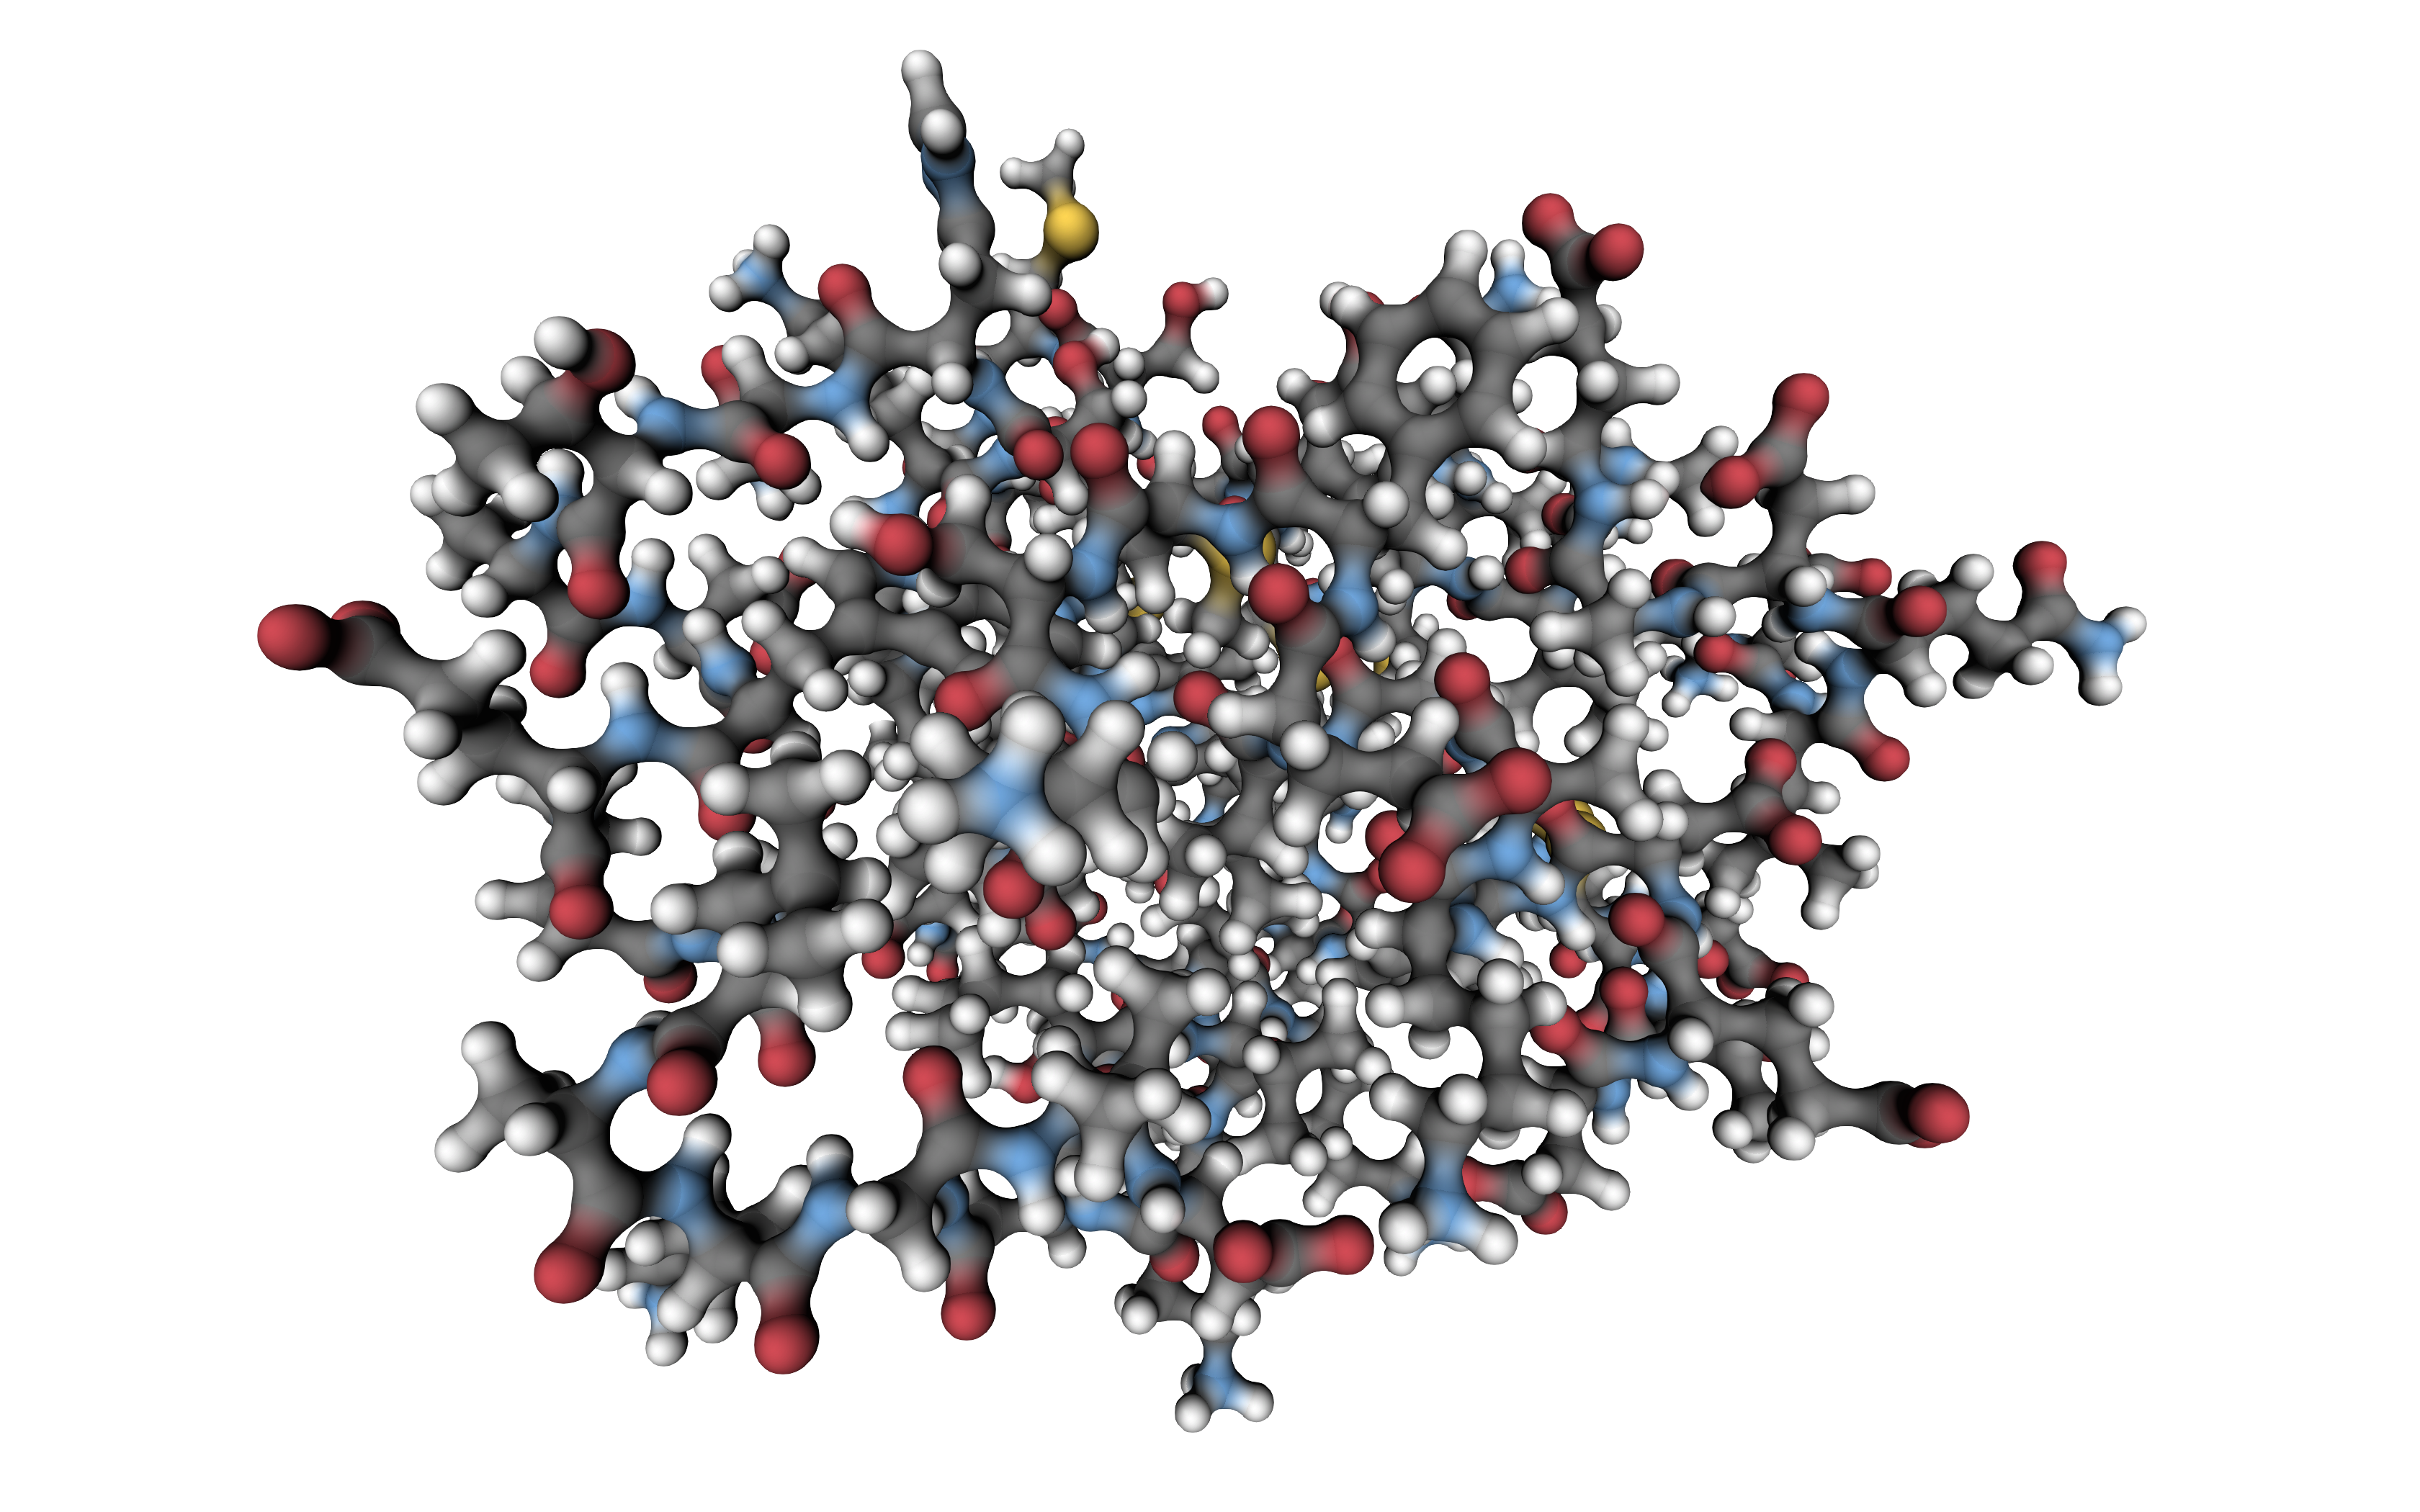
\includegraphics[width=\textwidth]{figures/ch1/1KX2}
		\caption{Illustration d'une protéine (1KX2, un mono-hème ferrocytochrome) produite avec le logiciel UnityMol~\cite{doutreligne2014unitymol}. Les atomes de carbone sont représentés en gris, ceux d'oxygène en rouge, d'hydrogène en blanc, et de soufre en jaune. Cette protéine est relativement petite, avec seulement 81 acides aminés, contre plusieurs centaines sur de nombreuses protéines ; de plus, ce mode de représentation, dans lequel les atomes ont un rayon inférieur à leur rayon de van der Walls, couramment utilisé, minimise l'occultation ; néanmoins, on constate qu'une très grande partie de la molécule est occulée par les atomes situés au premier plan. De surcroît, il s'agit ici d'une représentation \emph{in vacuo}, c'est-à-dire sans le solvant dans lequel une protéine se trouve généralement à l'état naturel.}
		\label{fig:1KX2}
	\end{figure}
	
	\paragraph{Modes de représentation.}
	Un atome n'est pas un objet au sens où on l'entend communément, dans un contexte macroscopique. S'il est courant de représenter un atome par une sphère, il n'a pas de rayon, de « coquille » et ce n'est qu'une représentation schématique de la réalité, utilisée pour communiquer une information. Autour du noyau de l'atome se trouve un nuage électronique où les électrons occupent de manière probabiliste certaines régions de l'espace. Pour représenter ce nuage électronique, on peut procéder comme sur la figure~\ref{fig:helium}.
	
	\begin{figure}[htb]
		\centering
		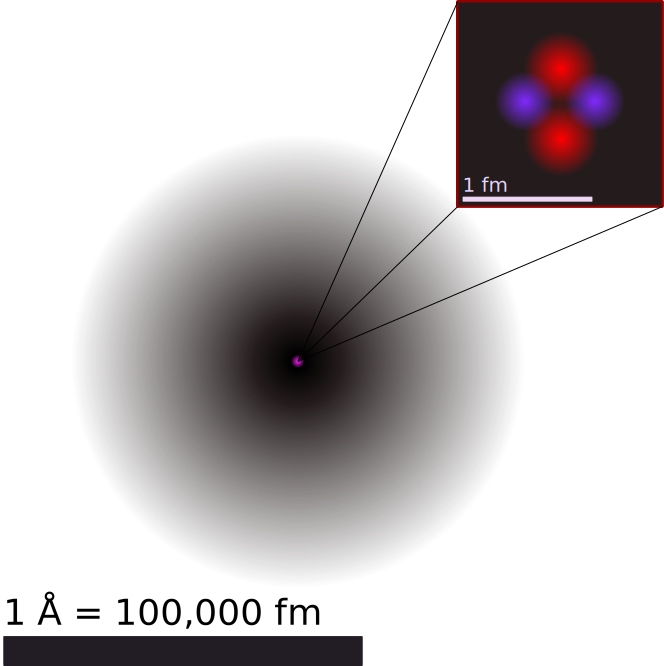
\includegraphics[width=\textwidth]{figures/ch1/helium}
		\caption{Illustration d'un atome d'hélium, représentant le noyau en rose et la distribution du nuage électronique en nuances de gris. Le noyau (en haut à droite) de l'hélium-4 est représenté de façon très schématisée. La barre noire en bas à gauche indique l'échelle, et mesure un \aa{}ngström, soit $0,1$ nanomètre. Crédit : \emph{Wikimedia Commons.}}
		\label{fig:helium}
	\end{figure}
	
	\begin{description}
		\item[CPK.] Blabla
		\item[Réglisse ou traits.] Blabla
		\item[VdW.] Blabla
		\item[\emph{Hyperballs}] Blabla
		\item[Structures secondaires] Blabla
		\item[Surface(s)] Blabla
	\end{description}
	
    
	\subsection{Dynamique moléculaire}
	Une simulation de dynamique moléculaire consiste à simuler, par un calcul numérique, le comportement d'un système moléculaire dans le temps. Celui-ci est modélisé par un système de particules, avec généralement une particule par atome. Des formules mathématiques permettent de modéliser les différences forces qui s'appliquent à chaque particule, et ces forces sont intégrées avec un pas de temps pour déterminer le comportement dynamique du système.
    
	\subsection{Simulations interactives}
	Besoin de steering, etc.
	L'interaction avec une simulation de dynamique moléculaire présente plusieurs difficultés majeures. Tout d'abord, le nombre de cibles potentielles est très élevé, avec au minimum plusieurs centaines d'objets, généralement plusieurs dizaines de milliers, voire plusieurs centaines de milliers, dans les cas les plus extrêmes. Ces cibles étant confinées dans un espace relativement petit, il en resulte de plus une densité élevée, voire très élevée (selon le mode de représentation.
	 occultaton, vitesse, prévisibilité, etc.
	
	\section{Contrôle de l'espace aérien}
	La figure~\ref{fig:airtraffic} représente un écran de contrôle du trafic aérien. Les trajectoires des avions sont (normalement) légèrement courbées ou rectilignes, ce qui les rend particulièrement prévisibles, et donc facilite considérablement la tâche de sélection, comme nous le verrons en détail plus loin. Cependant, selon le niveau de zoom et la quantité d'informations contextuelles affichées sur l'écran, le niveau d'occultation peut devenir très important. La vitesse des cibles dépend également du niveau de zoom, mais dans une relation inverse : plus l'échelle est grande, plus les mouvements des avions seront lents sur l'écran.
	
	\subsection{Applications civiles}
	Quantitativement, un avion de ligne atterrit à environ 250~km/h et ne dépasse pas 1000~km/h. Ses changements de direction sont très progressifs, généralement de l'ordre de deux degrés par seconde. Ils sont peu fréquents et généralement prévisibles car ils ont pour but d'emprunter des couloirs aériens, ou des trajectoires d'approche imposées aux abords des aéroports.

	\paragraph{}
	Il n'en va toutefois pas de même pour les hélicoptères, qui peuvent faire demi-tour en environ quatre secondes, voire moins. Cependant, les modèles civils dépassent rarement les 300 km/h. La fréquence des changements de direction dépend considérablement de la mission, elle peut être faible pour un simple transport d'un point A vers un point B, auquel cas la trajectoire de l'hélicoptère va tendre vers la ligne droite, ou assez importante dans le cas d'un hélicoptère de police fournissant une assistance aérienne pendant une course-poursuite.
	
	\subsection{Applications militaires (surveillance de l'espace aérien)}
	Les aéronefs militaires présentent des caractéristiques beaucoup plus variables, dans des intervalles nettement plus grands. La vitesse d'un avion de chasse, par exemple, peut atteindre 3000~km/h~\cite{mig31}. Il est beaucoup plus difficile d'obtenir des données chiffrées sur la maœuvrabilité de tels engins, mais il est du moins clair qu'un avion de chasse moderne peut changer de direction beaucoup plus brutalement qu'un avion de ligne, et certaines sources non officielles font état de capacités de l'ordre de 35\textdegree{}/s pour les meilleurs. La fréquence maximale à laquelle un avion peut changer de direction est également difficile à connaître avec certitude, mais une simple observation d'une démonstration en vol permet d'estimer que cette valeur est, grossièrement, de l'ordre d'un changement par seconde environ~\cite{rafdemo}. Indépendamment des capacités techniques des avions militaires, leurs missions peuvent précisément imposer la recherche de l'imprévisibilité (par exemple pour éviter les tirs ennemis) ce qui n'est généralement pas le cas dans le civil.
	
	\begin{figure}[ht]
		\centering
		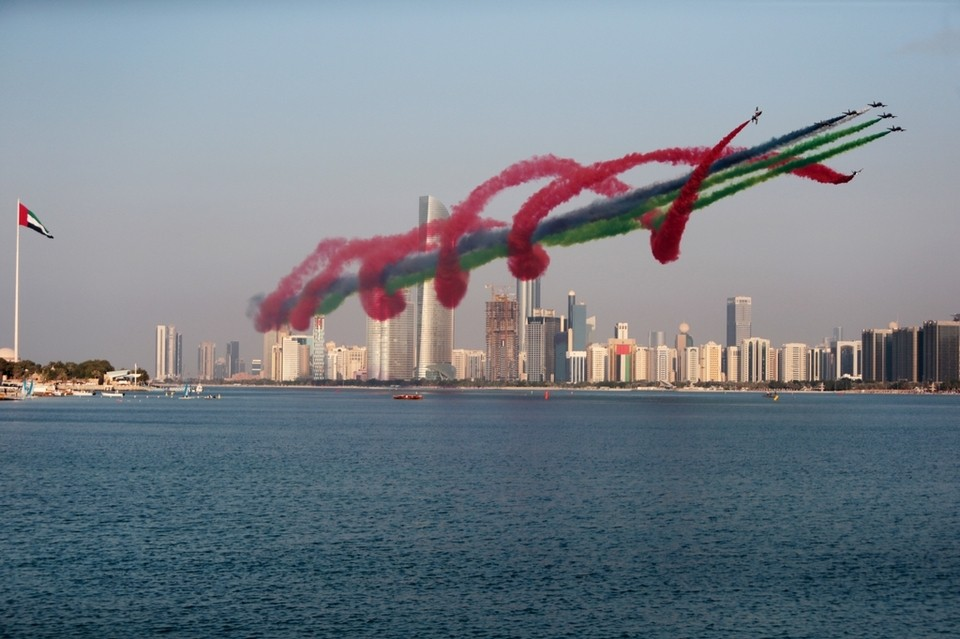
\includegraphics[width=\textwidth]{figures/AlFursan}
		\caption{La patrouille acrobatique émiratie \emph{Al Fursan}, avec ses trajectoires entremêlées mises en évidence par des traînées de fumée colorées. Crédit : The National UAE (\url{http://www.thenational.ae}).}
		\label{fig:alfursan}
	\end{figure}
	
	\paragraph{}
	De même, les hélicoptères militaires sont plus agiles que leurs homologues civils, sans qu'il soit aisé de quantifier cette différence. Comme pour les avions, leur comportement est susceptible d'être  Ils sont ausssi légèrement plus rapides, de quelques dizaines de km/h, notamment en piqué. Comme pour les avions, leurs missions impliquent souvent des trajectoires moins prévisibles.
	
	\paragraph{}
	Le cas des drones aériens, c'est-à-dire des aéronefs sans pilote embarqué (télécommandés ou autonomes) est peut-être le plus hétérogène. On trouve en effet des drones de très petite taille, mais aussi des modèles de plusieurs tonnes~\cite{reaper}. Leurs modes de sustentation sont très divers, leurs moyens de propulsion varient également, et de fait, leurs caractéristiques de vol sont extrêmement variables, des plus petits engins extrêmement manœuvrables jusqu'au plus gros, qui se comportent comme des avions. Au-delà de leurs caractéristiques de vol, certains drones sont délibérément conçus pour être utilisés en grandes quantités, en essaims~\cite{locust, alonso2016distributed, saska2014autonomous}, notamment pour submerger l'ennemi par le nombre. Cela implique une densité de cibles potentiellement très importante, avec les niveaux d'occultation qui en découlent.
	
	\begin{figure}[ht]
		\centering
		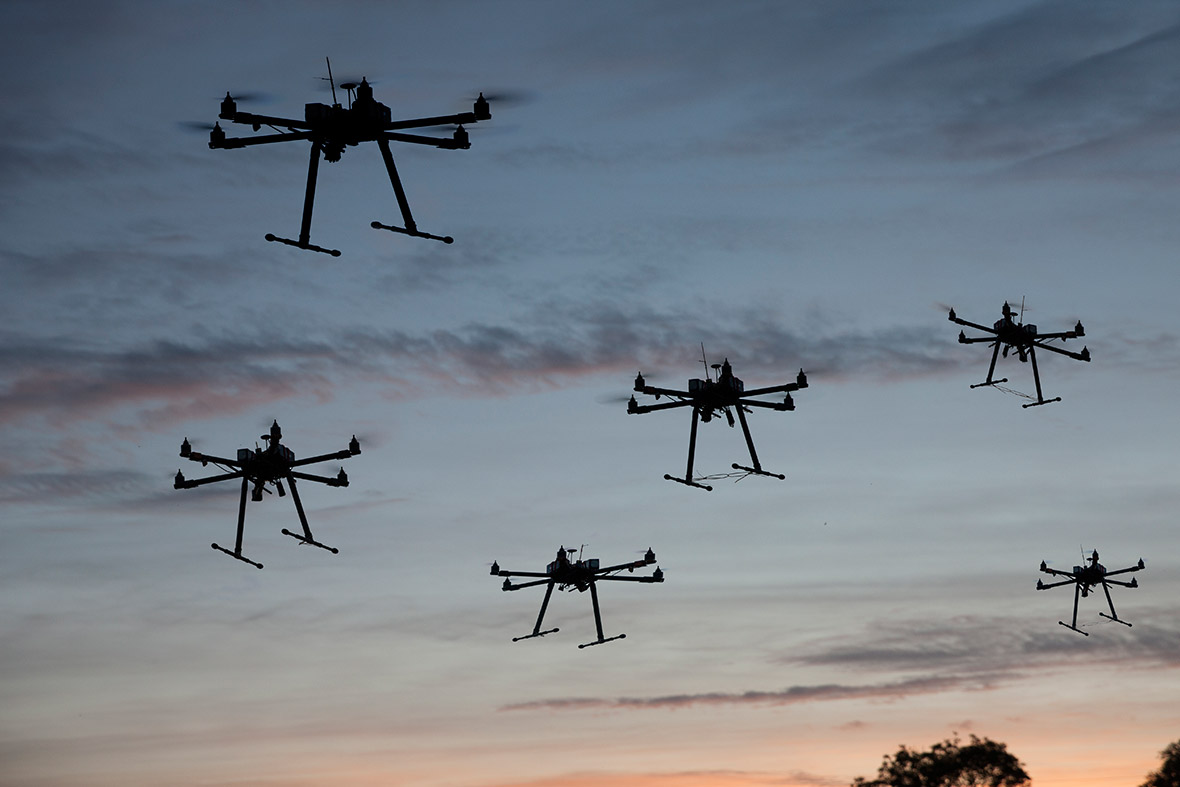
\includegraphics[width=\textwidth]{figures/swarm}
		\caption{Petit essaim de drones aériens. Crédit : \emph{International Business Times}.}
		\label{fig:swarm}
	\end{figure}
	
	\paragraph{}
	Dans une certaine mesure, le contrôle de la circulation des drones est également un enjeu pour le domaine civil, car ils peuvent évoluer (légalement ou non) près des aéroports. Cette pratique peut représenter un risque de sécurité, et des arrêtés ont été pris par le Ministère de l'écologie et du développement durable pour les prévenir, comme le rappelle notamment l'Union des Aéroports Français~\cite{dronesuaf}.
	
	\paragraph{}
	Les drones représentent aussi un risque sécuritaire civil généralisé :
	
	\begin{displayquote}
	C'est un mode d'action inédit contre des forces françaises. Le camp militaire d'Erbil, qui abrite des peshmergas et des commandos français au Kurdistan irakien, a été le théâtre d'une explosion sans précédent le 2 octobre dernier. Celle d'un drone, piégé par le groupe Etat islamique. Bilan : deux combattants kurdes tués, et deux commandos parachutistes de l'armée de l'air française grièvement blessés.
	
	[\ldots{}]
	
	« On ne peut pas faire grand-chose », constate avec amertume auprès de LCI Jean-Vincent Brisset, général de brigade aérienne. Ce directeur de recherche à l’IRIS l'assure : « C'est quelque chose d'assez terrifiant pour les services de sécurité. Il est horriblement compliqué de stopper un drone qui, par exemple, chercherait à s'attaquer à un responsable politique en plein discours. » Pour preuve, la scène surréaliste à laquelle avaient assisté ceux qui écoutaient Angela Merkel, il y a trois ans à Dresde. Durant son intervention, la chancelière avait observé l’atterrissage surprise d’un appareil au pied de la tribune.~\cite{brisset}

	
	\end{displayquote}
	
	\paragraph{}
	La surveillance de l'espace aérien concerne également divers types de missiles (de croisière, balistiques, etc.). Leurs caractéristiques détaillées sont généralement au moins aussi secrètes que celles des avions de chasse, mais on sait néanmoins qu'ils peuvent être à la fois hypersoniques (c'est-à-dire dépasser Mach~5) et manœuvrables à de telles vitesses~\cite{missiles}, comme le missile BrahMos-II dont une maquette est représentée sur la figure~\ref{fig:brahmos}.
	
	\begin{figure}[ht]
		\centering
		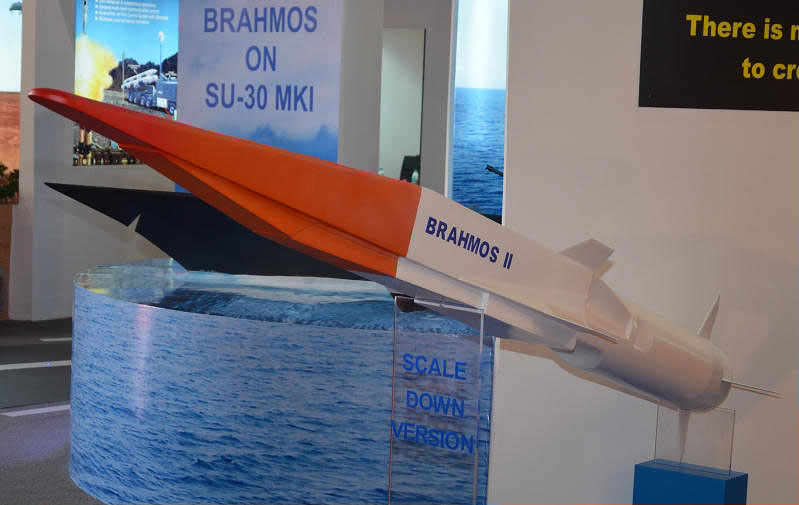
\includegraphics[width=\textwidth]{figures/brahmos-II}
		\caption{Maquette du missile hypersonique russo-indien BrahMos-II, en cours de développement. Crédit : Pakistan Defence (\url{http://defence.pk}).}
		\label{fig:brahmos}
	\end{figure}
	
	\paragraph{}
	En situation réelle, un espace aérien pourrait tout à fait contenir des véhicules et autres engins volants de tous les types sus-cités, des essaims de drones très manœvrables jusqu'aux missiles balistiques les plus rapides. Un système de contrôle interactif devrait donc être assez souple pour permettre la sélection de cibles de natures très différentes.
	On peut noter que les engins volants militaires ont vocation à chercher à éviter d'être détectés, soit en étant naturellement furtifs, soit en volant à très basse altitude et en tirant parti du relief naturel. Il en résulte qu'ils peuvent n'apparaître sur les écrans de contrôle que lorsqu'ils sont déjà très proches de lieux à protéger, et peuvent éventuellement disparaître de ces écrans, offrant une fenêtre temporelle restreinte pour l'interaction.
	
	\subsection{Observations}
	Qu'il s'agisse d'applications civiles ou militaires, cette tâche est critique, puisque de nombreuses vies sont en jeu. Selon l'application, il peut donc y avoir des contraintes fermes et spécifiques, soit sur le temps de sélection maximal acceptable (contrainte de temps-réel) soit sur le taux d'erreur, ou encore sur les niveaux de zoom, etc.

	Les systèmes de contrôle aérien dont nous avons connaissance sont tous en deux dimensions. Pour des engins volants, cela implique nécessairement une perte d'informations. Une technique de sélection suffisamment performante pourrait rendre envisageable l'utilisation d'un système en 3D. Cela permettrait par exemple de mieux déterminer si deux avions qui paraissent dangereusement proches dans le plan le sont réellement dans l'espace, ou de pouvoir choisir un objet parmi plusieurs évoluant aux mêmes coordonnées 2D, mais à des altitudes différentes, ou tout simplement d'avoir une meilleure représentation et perception générales de la situation.

	\begin{figure}[ht]
		\centering
		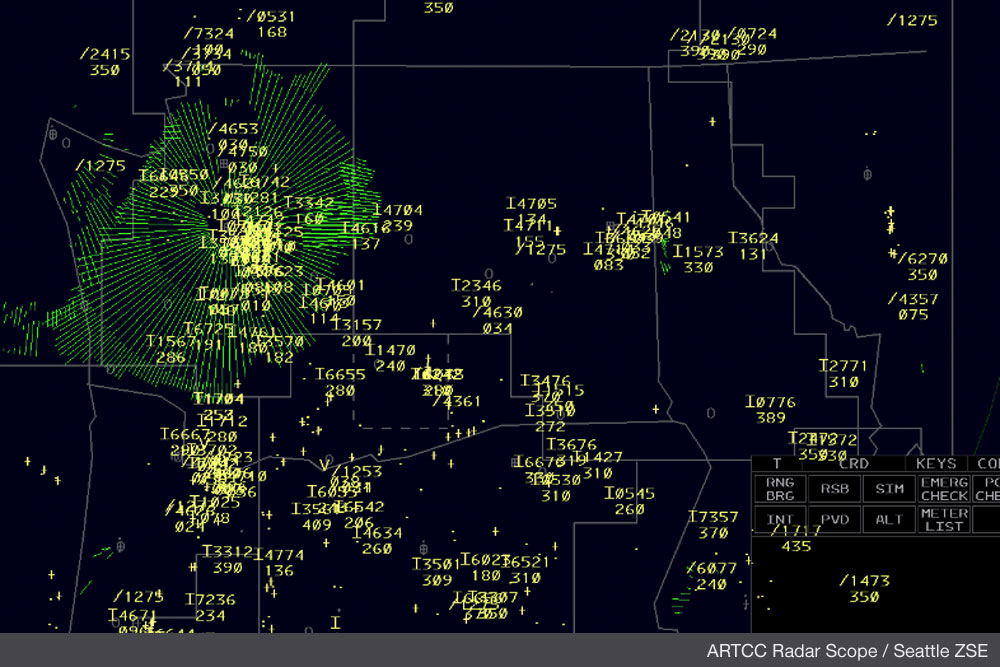
\includegraphics[width=\textwidth]{figures/Radar-Scope-ZSE}
		\caption{Écran de contrôle du trafic aérien. Toutes les informations, qui portent pourtant sur un espace tridimentionnel, sont représentées sur le même plan, avec une densité telle que certaines indications écrites sont illisible. Crédit : \emph{Bold Method}.}
		\label{fig:airtraffic}
	\end{figure}
	
	\section{Contrôle de l'espace maritime}
	\subsection{Enjeux}
	La figure~\ref{fig:channel} représente un écran de contrôle du trafic maritime en Manche. Fondamentalement, il s'agit d'un problème très similaire à celui du contrôle du trafic aérien, car il s'agit dans les deux cas de surveiller et organiser un espace fluide. Comme dans les airs, les enjeux sont à la fois militaires et civils. Les bâtiments militaires (\emph{a fortiori} s'ils sont potentiellement hostiles) doivent en effet être détectés le plus tôt possible et suivis tant qu'ils sont dans un espace d'intérêt défini, mais il faut également surveiller les bâtiments civils.
	
	\paragraph{}
	En effet, au-delà des activités commerciales normales qui font l'objet de contrôles douaniers, la mer abrite des activités illégales diverses, incluant tous types de trafics (contrebande, œuvres d'art, drogue, armes, êtres humains) mais aussi la piraterie ou des activités liées au terrorisme.
	Le fret maritime mondiale représentant près de 10 milliards de tonnes, on mesure l'ampleur et l'importance du défi à l'échelle planétaire~\cite{unctad}.
	
	
	\begin{figure}[ht]
		\centering
		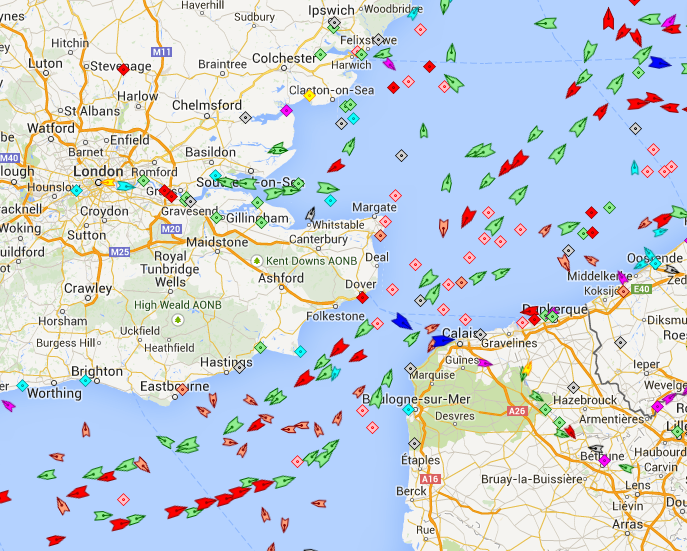
\includegraphics[width=\textwidth]{figures/channel}
		\caption{Écran de contrôle représentant les navires utilisant le Système d'identification automatique (SIA) en Manche. Ce système n'étant obligatoire que sur les navires de jauge brute supérieure à 300 effectuant des voyages internationaux, ce n'est qu'une représentation partielle du trafic à cet instant. Crédit : \emph{Arlo Maritime}.}
		\label{fig:channel}
	\end{figure}
	
	\subsection{Difficultés}
	La plupart des navires se déplacent à la surface de l'eau. Par conséquent, leur représentation dans le plan sur un écran de contrôle n'implique généralement pas de perte d'information significative, contrairement au cas aérien. Toutefois, les sous-marins peuvent plonger à plusieurs centaines de mètres. S'ils représentent une très petite minorité des navires en circulation, leur détection revêt une importance militaire critique.
	
	\paragraph{}
	De fait, le problème de l'affichage planaire d'information tridimensionnelles demeure, même s'il est moins prégnant. Les navires sont en moyenne bien plus lents que les aéronefs, mais certains bateaux de type \emph{go-fast} peuvent dépasser les 150~km/h. Ces navires étant fréquemment utilisés par les trafiquants de drogue pour échapper aux garde-côtes, il est particulièrement important de pouvoir les détecter et les contrôler.
	
	\paragraph{}
	Comme souvent pour les tâches de ce type, la densité de cibles dépend du niveau de zoom, qui peut résulter d'un choix de l'utilisateur, ou d'une contrainte (l'obligation d'avoir en permanence une zone donnée affichée, par exemple). La densité peut donc varier et, potentiellement, être très élevée. Elle devient particulièrement problématique lorsque l'on souhaite afficher des informations contextuelles à propos des navires, ou d'un sous-ensemble de ceux-ci. Ces informations peuvent concerner le type du navire, son pavillon, son propriétaire, son équipage, son origine, sa destination (connue ou présumée) ses escales, sa cargaison, etc., ainsi que les éventuelles précédentes valeurs de toutes ces données.
	
	\paragraph{}
	Ces informations revêtent une importance particulière lorsqu'il est nécessaire aux autorités de faire la différence entre un bateau effectuant un simple voyage de plaisance et une embarcation susceptible d'être engagée dans une activité criminelle. Un groupe de \emph{speedboats} filant à vive allure vers une destination donnée peut tout aussi bien être un groupe d'amis en promenade qu'une bande de trafiquants de drogue. Il est donc nécessaire aux agents de contrôle de l'espace maritime de disposer d'un maximum d'informations le plus vite possible pour déterminer s'il est nécessaire d'ordonner l'interception de ces bateaux.
	
	\paragraph{}
	La figure~\ref{fig:lincoln} illustre un cas de forte densité locale de navires, avec des cibles de haute importance stratégique de surcroît. Près des ports, la densité peut être plus élevée encore, même si les navires concernés sont moins préoccupants pour les autorités. Il leur est toutefois nécessaire de garantir la circulation fluide et sûre de ces navires, et de veiller à ce que personne ne tire parti de cette forte densité à des fins illicites ou criminelles.
	
	\begin{figure}[ht]
		\centering
		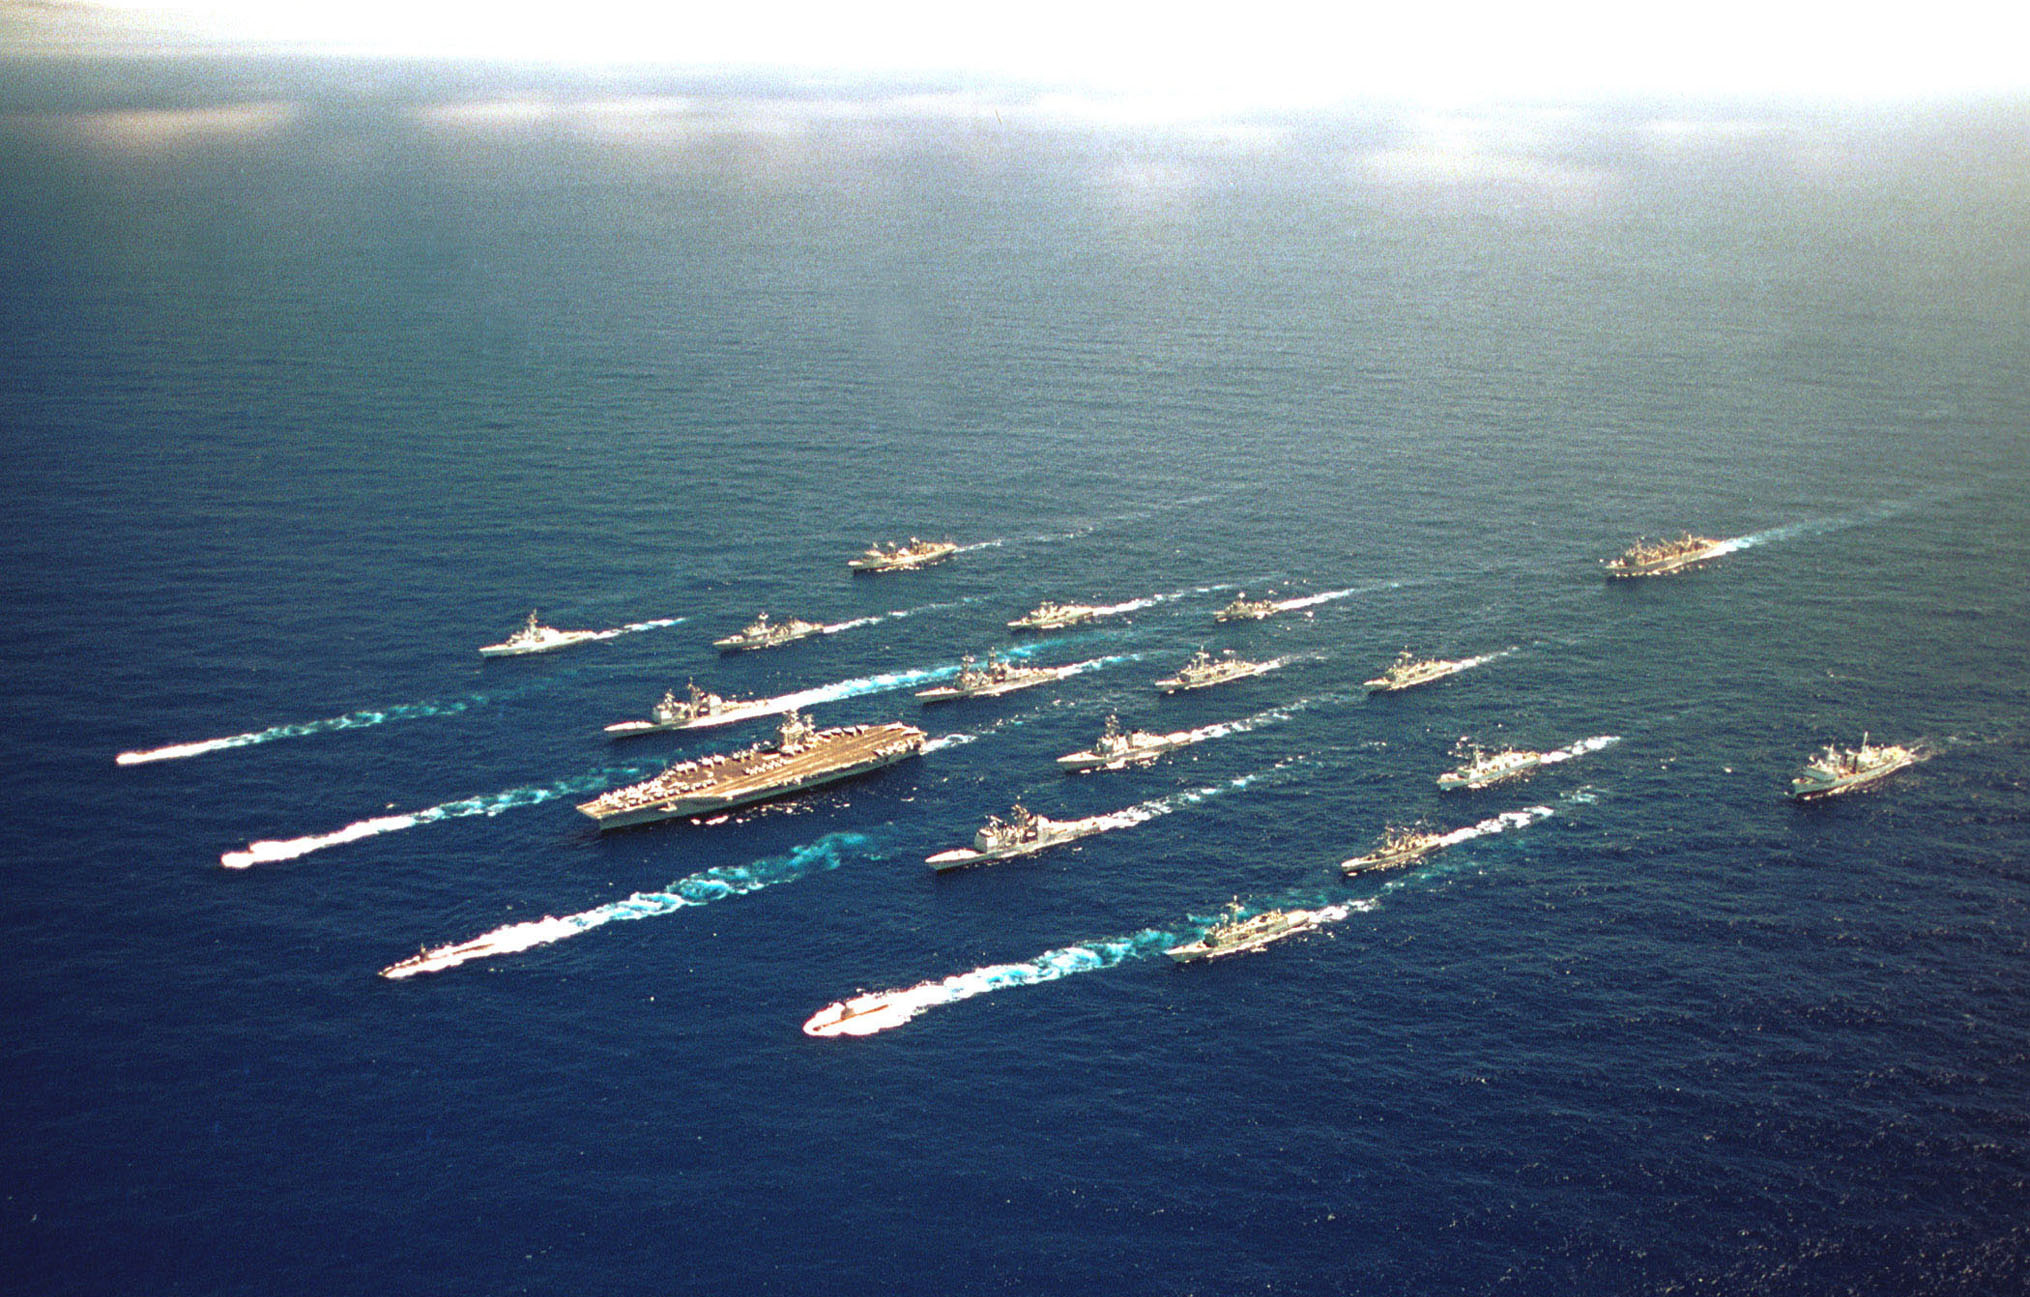
\includegraphics[width=\textwidth]{figures/lincoln}
		\caption{Même dans des eaux relativement vides, la densité de navries peut être élevée localement. C'est généralement le cas quand un groupe aéronaval est présent, comme ici, avec le groupe aéronaval Abraham Lincoln, photographié en 2000. Il est de plus capital dans ce cas d'identifier clairement tous les navries présents, compte tenu de leur importance militaire. Crédit : \emph{Gabriel Wilson, via Wikimedia}.}
		\label{fig:lincoln}
	\end{figure}
	
	\section{Vidéo-surveillance}
	La vidéo-surveillance s'applique aussi bien aux foules dans les lieux publics ou sensibles qu'à la voirie, où peuvent circuler des véhicules de types divers. Un agent de sécurité en charge de visionner un flux de vidéo-surveillance pourrait avoir à sélectionner une personne, par exemple pour obtenir des informations sur celle-ci grâce à la reconnaissance faciale, ou un véhicule, pour les mêmes raisons, par exemple grâce à sa plaque d'immatriculation. Quelle que soit la nature de la cible, sa sélection pourrait avoir pour but de zoomer dessus, de verrouiller une caméra robotisée afin qu'elle la suive, ou de la désigner à des forces de sécurité sur le terrain pour qu'elles interviennent physiquement.
	
	\paragraph{}
	La vitesse d'un être humain à pied est inférieure à 45~km/h. Les changements de direction peuvent aller jusqu'au demi-tour, et leur fréquence est très variable selon la tâche accomplie. On peut supposer que cette fréquence est au plus de l'ordre de quelques Hz, en pratique généralement moins.

	\paragraph{}	
	Sur la voie publique, un véhicule motorisé n'est pas censé dépasser 130~km/h, exception faite de ceux qui enfreignent le code de la route. Mais, soit à cause de l'infraction en question, soit parce qu'ils l'enfreignent pour fuir après des délits ou crimes plus graves, ces véhicules-là peuvent justement faire l'objet d'une attention particulière de la part des forces de l'ordre. Dans ces cas-là, la vitesse d'un véhicule peut dépasser les 300~km/h~\cite{speeding}.
	
	Les changements de direction dépendent évidemment de la vitesse. En ville, à moins de 50~km/h, une automobile peut effectuer un virage à 90 degrés dans un laps de temps de l'ordre de la seconde si sa vitesse est réduite, mais elle est contrainte à des courbes beaucoup plus douces lorsqu'elle se déplace rapidement, par exemple sur une autoroute.
	
	La fréquence des changements de direction dépend également de la vitesse, tant pour des raisons physiques que du fait du tracé des trajets communément effectués. En milieu urbain dense, on peut considérer qu'un véhicule va changer de direction, de façon plus ou moins prononcée, à une fréquence de l'ordre de 0,1~Hz, sachant qu'en cas de nécessité, cette fréquence peut être nettement plus élevée.
	
	\paragraph{}
	En plus des piétons et des automobiles, la vidéo-surveillance s'applique à tous les véhicules et moyens de déplacement susceptibles d'être utilisés dans l'espace public : patins à roulettes, skateboards de tous types, bicyclettes, motocyclettes, etc. Les caractéristiques du mouvement de ces moyens de transport sont diverses, mais généralement comprises dans les intervalles formés par les piétons et les automobiles. Il est donc important qu'une technique de sélection puisse non seulement gérer les valeurs extrêmes de vitesse, d'angle et de fréquence de changements de direction, mais également les diverses combinaisons de ces valeurs qui peuvent se présenter simultanément.
	
	\paragraph{}
	Dans certains cas, par exemple au cours de manifestations publiques ou de concerts, les individus filmés peuvent devenir quasi statiques, mais très nombreux et confinés dans un espace réduit. Il en résulte une densité de cibles potentielles et un niveau d'occultation très élevés. Dans ces circonstances, la vidéo-surveillance 
	
	\begin{figure}[ht]
		\centering
		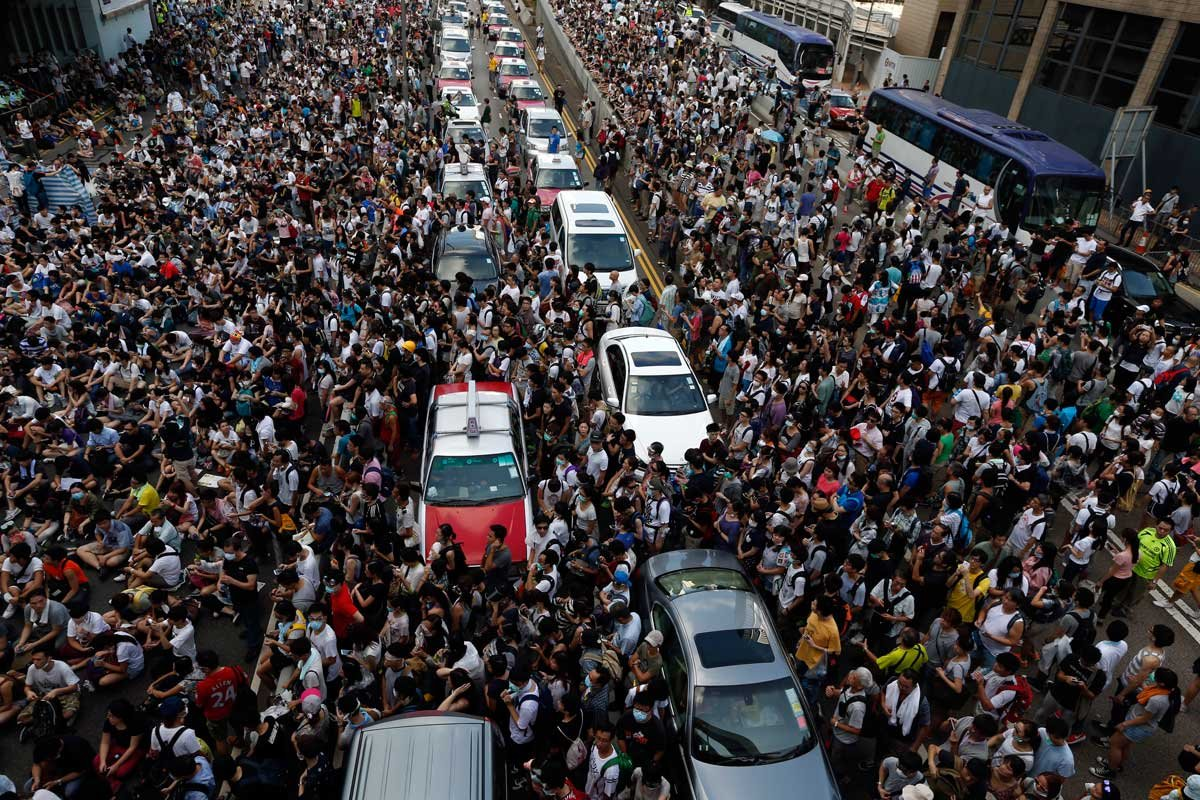
\includegraphics[width=\textwidth]{figures/crowdhk}
		\caption{Foule de manifestants à Hong-Kong. Mouvement très faible, mais densité très élevée. Crédit : \emph{Business Insider}.}
		\label{fig:crowdhk}
	\end{figure}
	
	\begin{figure}[ht]
		\centering
		\includegraphics[width=\textwidth]{figures/crowdacdc}
		\caption{Foule à un concert du groupe AC/DC. Mouvement presque nul, mais densité extrêmement élevée. Crédit : \emph{SHP Online}.}
		\label{fig:crowdacdc}
	\end{figure}
	
	
	
	\section{Analyse de processus complexes}
	Mélange d'humains, de machines, espaces 3D, multiplicité d'objets, etc.
	
	\section{Retransmissions d'événements sportifs ou artistiques}
	Les retransmissions d'événements sportifs présentent un potentiel d'interactivité intéressant, nécessitant souvent la sélection de cibles mobiles. Il peut être utile, par exemple, de sélectionner un joueur de football pour afficher ses statistiques. Pour les mêmes raisons, un ballon ou une balle peut être une cible, de même que certains éléments du terrain de jeu, qui sont physiquement fixes mais peuvent être mobiles à l'écran du fait des mouvements de caméra. La nature du mouvement de ces cibles varie nécessairement d'un sport ou d'un jeu à l'autre.
	
	\paragraph{}
	Certains sports d'équipe comme le football, le hockey sur glace ou le basket-ball sont caractérisés par des cibles potentielles relativement nombreuses, mobiles, et dont les mouvements ne sont pas toujours très prévisibles. Les mouvements d'humains à pieds obéissent aux règles habituelles, mais dans un cadre sportif, ils peuvent être sur des patins à glace, des bicyclettes, des skis, etc., sans parler des sports hippiques ou mécaniques. Dans ces derniers cas, les mouvements sont souvent plus prévisibles, mais aussi nettement plus rapides, avec en plus une certaine tendance des cibles à être très proches les unes des autres, ce qui augmente la probabilité d'erreur de sélection.
	
	\paragraph{}
	Les divers projectiles utilisés en sports (balles, ballons, volants, palets, etc.) sont généralement beaucoup plus petits et rapides que les joueurs, ce qui en fait des cibles très difficile. D'un autre côté, il n'y a généraelement qu'un seul projectile de ce type par match, donc dans la mesure du possible, un raccourci dédié serait probablement une option préférable à l'utilisation d'une technique de sélection libre, fût-elle assistée.
	
	\begin{figure}[ht]
		\centering
		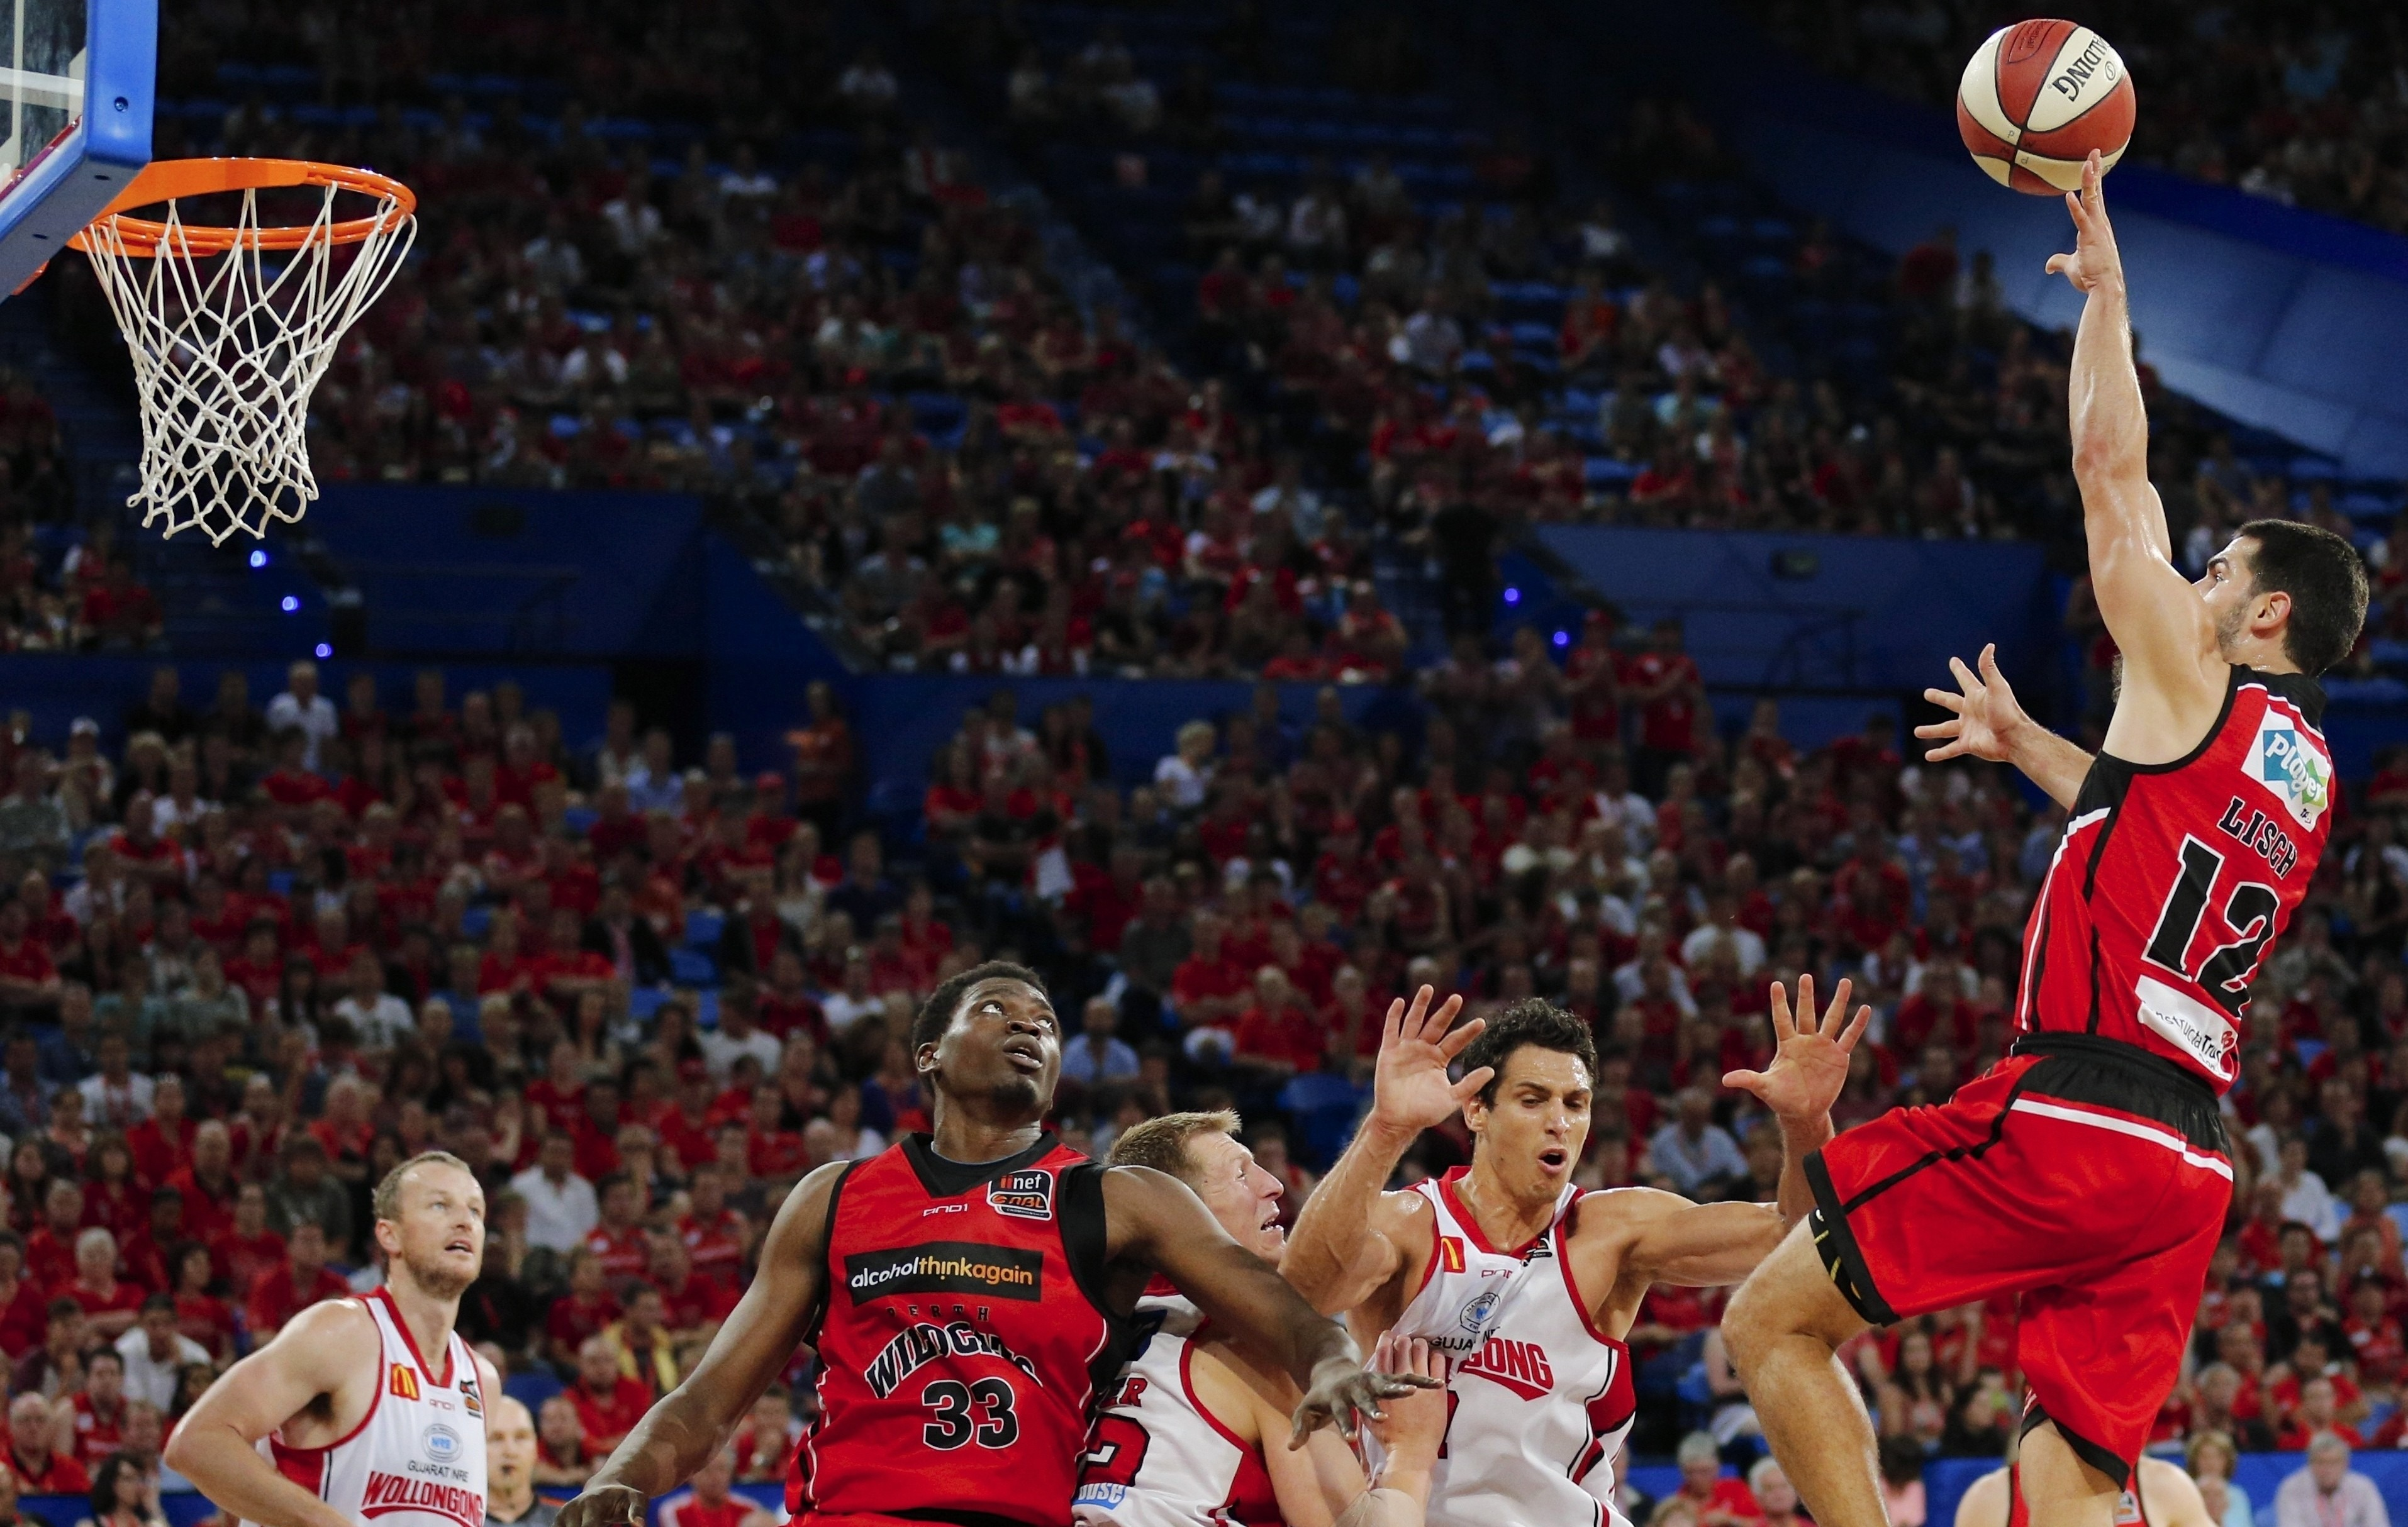
\includegraphics[width=\textwidth]{figures/basket}
		\caption{Match de basket-ball. Les joueurs sont peu nombreux, mais leurs mouvements sont vifs, horizontaux comme verticaux, et imprévisibles. Ils sont de plus très près les uns des autres et s'occultent mutuellement, \emph{a fortiori} quand ils sont filmés depuis le côté. Le ballon lui-même peut être une cible. Crédit : \emph{Weekend Notes}.}
		\label{fig:basketball}
	\end{figure}
	
	\section{Jeux vidéo}
	La sélection ou le pointage de cibles mobiles est une tâche que l'on retrouve dans de très nombreux jeux vidéo, appartenant à un nombre important de catégories. On peut notamment citer les jeux de tir (\emph{Fist-person Shooters}, ou FPS, comme \emph{Doom}, \emph{Counter-Strike}\ldots{}), les jeux de rôle d'action (\emph{Action role-playing games}, ou ARPG, comme \emph{The Witcher}, \emph{The Elder Scrolls}, voire \emph{Deus Ex}\ldots{}) les jeux de gestion (\emph{Anno}, \emph{Civilization}\ldots{}) ou de stratégie et tactique militaire (les catégories \emph{Real-time strategy} ou RTS, dans laquelle on trouve des jeux comme \emph{Starcraft} ou \emph{Age of Empires}, et \emph{Real-time tactics} ou RTT, avec \emph{Total War} ou \emph{World in Conflict}\ldots{}), les simulateurs de vol de combat (réalistes ou non, comme \emph{X-Plane}, \emph{IL-2 Sturmovik}, \emph{Elite: Dangerous}\ldots{}) ainsi que les jeux de type arène de bataille en ligne multijoueur (\emph{Multiplayer online battle arena}, ou MOBA, tels que \emph{League of Legends} ou \emph{DOTA~2}).
	
	D'un type de jeu à l'autre, la sélection de cibles varie à la fois du fait de la nature des cibles et parce que la tâche elle-même n'est pas vue de la même façon. Si elle est un élément essentiel des mécanismes du jeu dans certains genres, avec une valeur ludique propre, dans d'autres, elle est purement utilitaire, comme nous allons le voir dans les sous-sections suivantes.
	
	\subsection{Jeux de tir (FPS) et jeux de rôle d'action (ARPG)}
	Attendu que dans les FPS, la visée est précisément le cœur du jeu, et censée être difficile, les développeurs seraient probablement peu enclins à intégrer des techniques la facilitant, car cela diminuerait l'intérêt ludique de leur œuvre. Dans un jeu de rôle classique, c'est plutôt l'inverse. Les capacités du (des) personnage(s) contrôlé(s) par le joueur dépendent de l'expérience accumulée depuis le début du jeu, l'expérience étant ici une ressource précisément quantifiée, sous forme de points. Ces points sont ensuite investis dans des attributs (force, dextérité, endurance, intelligence\ldots{}) ou compétences (combat à mains nues, tir au fusil, persuasion, furtivité, magie de types divers\ldots{}). Souvent, les performances de visée d'un personnage dépendent uniquement de ses attributs et compétences, et non de la dextérité du joueur, qui n'a pas forcément besoin de désigner les cibles (le personnage les choisissant automatiquement) ou qui peut le faire pendant que l'action du jeu est en pause.
	
	\paragraph{}
	Mais il existe aussi une catégorie intermédiaire, les jeux de rôle d'action (ARPG). Les détails varient d'un jeu à l'autre, mais en général, le joueur est directement responsable des mouvements de ses personnages, mais les attributs et compétences du personnage ont une influence sur ses performances finales. Ce principe peut être mis en œuvre de diverses façons. En ce qui concerne le tir avec une arme (pistolet, arc, fusil\ldots{}) trois options, pas forcément mutuellement exclusives, sont couramment retenues :
	\begin{description}
		\item[Dispersion.] Quand les compétences de tir du personnage sont faibles, le réticule de visée est agrandi, ce qui indique au joueur que le cône de dispersion est large. À mesure que les compétences du personnage augmentent, le réticule et le cône se resserrent.
		\item[Perturbations.] Le curseur et le cône de dispersion peuvent être constants, mais ils bougent même lorsque le joueur ne touche pas à son périphérique de saisie. Celui-ci doit donc compenser ces mouvements pour viser correctement. À mesure que les compétences du personnage augmentent, ces mouvements diminuent, et peuvent finir par disparaître.
		\item[Recul.] Une arme qui tire un projectile a généralement un certain recul. Celui-ci n'a pas d'influence sur la précision du premier tir, mais sur tous les suivants. Dans un jeu vidéo, il est généralement simulé par un mouvement du curseur après le tir, habituellement vers le haut, avec en plus une composante horizontale, qui peut être aléatoire. On peut diminuer cet effet de recul quand les compétences du personnage croissent.
	\end{description}

	\paragraph{}
	Ces mécanismes permettent d'obtenir une difficulté de tir qui dépend du joueur, puisqu'il doit tout de même viser, mais les compétences du personnage jouent sur la difficulté de la tâche. On remarque qu'il s'agit toujours de gêner le joueur, de lui imposer un handicap qui diminue quand les compétences de ses personnages augmentent. Au final, le joueur reste borné par sa propre dextérité, comme dans un FPS classique.
	
	\paragraph{}
	Une autre technique, utilisée par les récents opus de la série \emph{Fallout} (désormais produite par Bethesda Studios) appelée \emph{Vault-Tec Assisted Targeting System}, ou V.A.T.S, consiste à arrêter ou considérablement ralentir le temps, pour permettre au joueur de désigner ses cibles, que le personnage attaquera ensuite automatiquement. Cette opération se fait en échange de << points d'action >>. L'inconvénient majeur de cette solution est la perte du temps-réel, et l'impact négatif sur l'immersion qui y est associé. De plus, le caractère automatique de l'attaque, une fois les cibles désignées, rend l'opération totalement indépendante de la dextérité du joueur, ce qui d'une part est une déviation du paradigme de l'ARPG, et d'autre part peut diminuer l'intérêt ludique du combat.
	
	\paragraph{}
	On pourrait imaginer, à la place ou en complément de ces approches, d'apporter au joueur une assistance à la visée. Une telle technique d'aide à la sélection devrait être paramétrable dans son << intensité >>, c'est-à-dire qu'il devrait lui être possible d'apporter au joueur une assistance plus ou moins prononcée, selon un paramètre donné. Ce paramètre pourrait être (dérivé de) la compétence de tir du personnage. Ainsi, un joueur contrôlant un personnage expert en tir serait capable d'abattre des cibles très difficiles, conformément à l'image du personnage telle qu'elle est véhiculée par le jeu, mais le joueur resterait l'acteur principal de l'opération, sans ralentissement ou suspension du temps.
	
	\begin{figure}[ht]
		\centering
		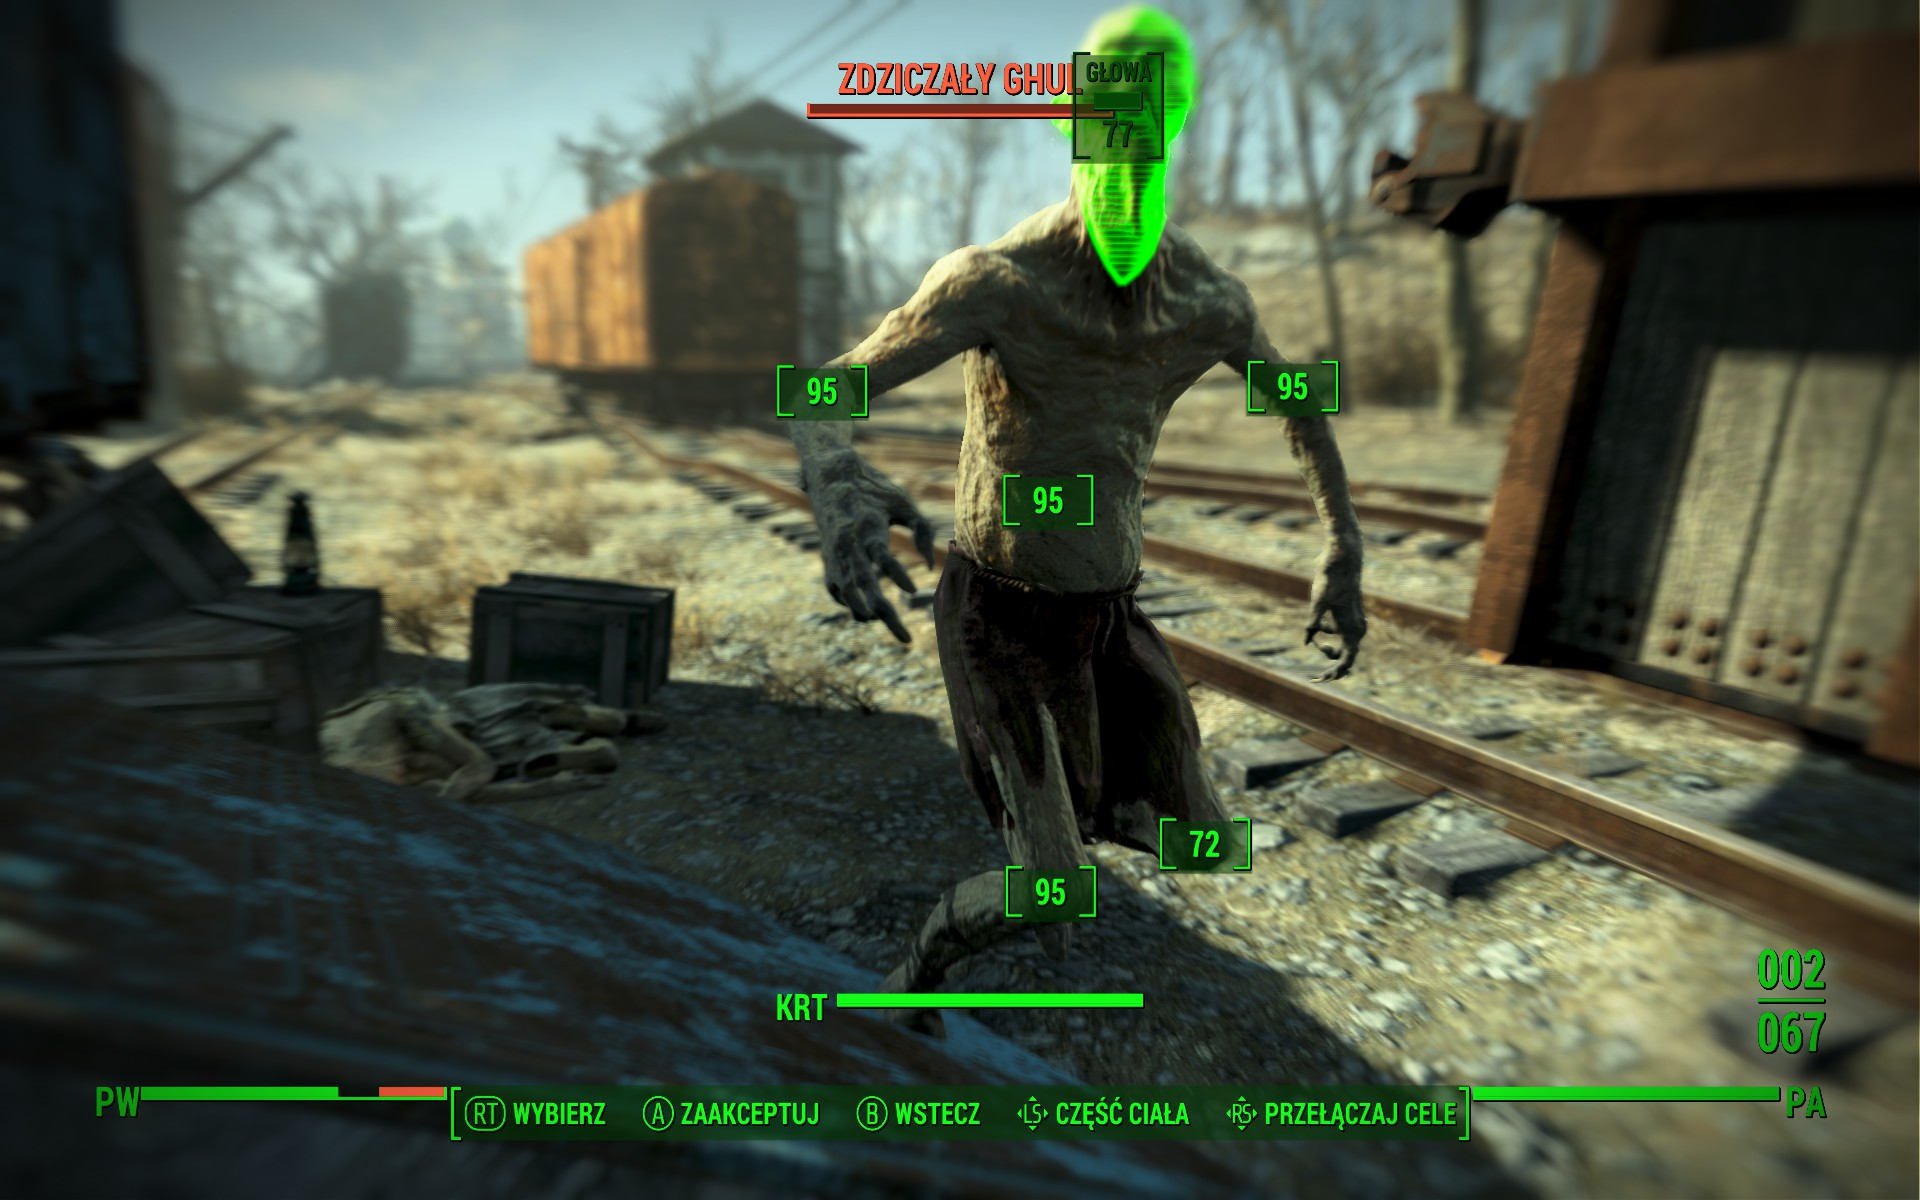
\includegraphics[width=\textwidth]{figures/f4vats}
		\caption{Dans l'ARPG \emph{Fallout 4}, le système V.A.T.S. permet ici au joueur de cibler tranquillement la tête de cette créature, pendant que le temps est ralenti. Le tir aura une probabilité de succès de 77~\%{}, dérivée des compétences de tir du personnage contrôlé, et des circonstances du combat à cet instant précis. Crédit : \emph{Spider's Web}.}
		\label{fig:f4vats}
	\end{figure}
	
	\subsection{Jeux de gestion, de stratégie (RTS) et de tactique (RTT)}
	Dans ce que nous appellerons, pour simplifier, les jeux de gestion (en y incluant les RTS et RTT) le but est de mener un organisme (d'une petite entreprise à une civilisation) vers la prospérité, ou une armée vers la victoire. Ces genres mettent l'accent sur la réflexion tactique et stratégique, la gestion des ressources naturelles et humaines, l'organisation logistique, l'utilisation astucieuse du terrain, l'art de la feinte, etc. S'il est fréquemment nécessaire de sélectionner des cibles dans ces jeux, ce n'est pas une fin en soi, ou un objectif conçu comme ayant une valeur ludique. Il s'agit de sélectionner des unités amies pour leur donner des instructions, ou des unités ennemies pour les désigner comme cibles à attaquer. Au contraire, la tâche de sélection fait perdre du temps au joueur, du temps qui pourrait être utilisé pour organiser ses resources et forces, ou tout simplement pour réfléchir.
	
	\paragraph{}
	Par conséquent, une technique de sélection facilitant cette tâche autant que possible serait probablement bénéfique en recentrant ces jeux sur leurs cœurs. Dans les jeux de gestion, les cibles peuvent être extrêmement nombreuses. Dans \emph{Cossacks~2: Napoleonic Wars}, par exemple, une bataille peut engager jusqu'à 64~000 unités, et la situation devient suffisamment assez délicate à gérer pour pousser les joueurs à mettre le jeu en pause, le temps de donner des instructions aux unités~\cite{cossacks2}. Il est évident que si cette solution est acceptable (quoique loin d'être idéale) dans un jeu opposant une intelligence artificielle au joueur humain, elle vient beaucoup plus gênante dans un contexte multijoueur.
	
	
	\begin{figure}[ht]
		\centering
		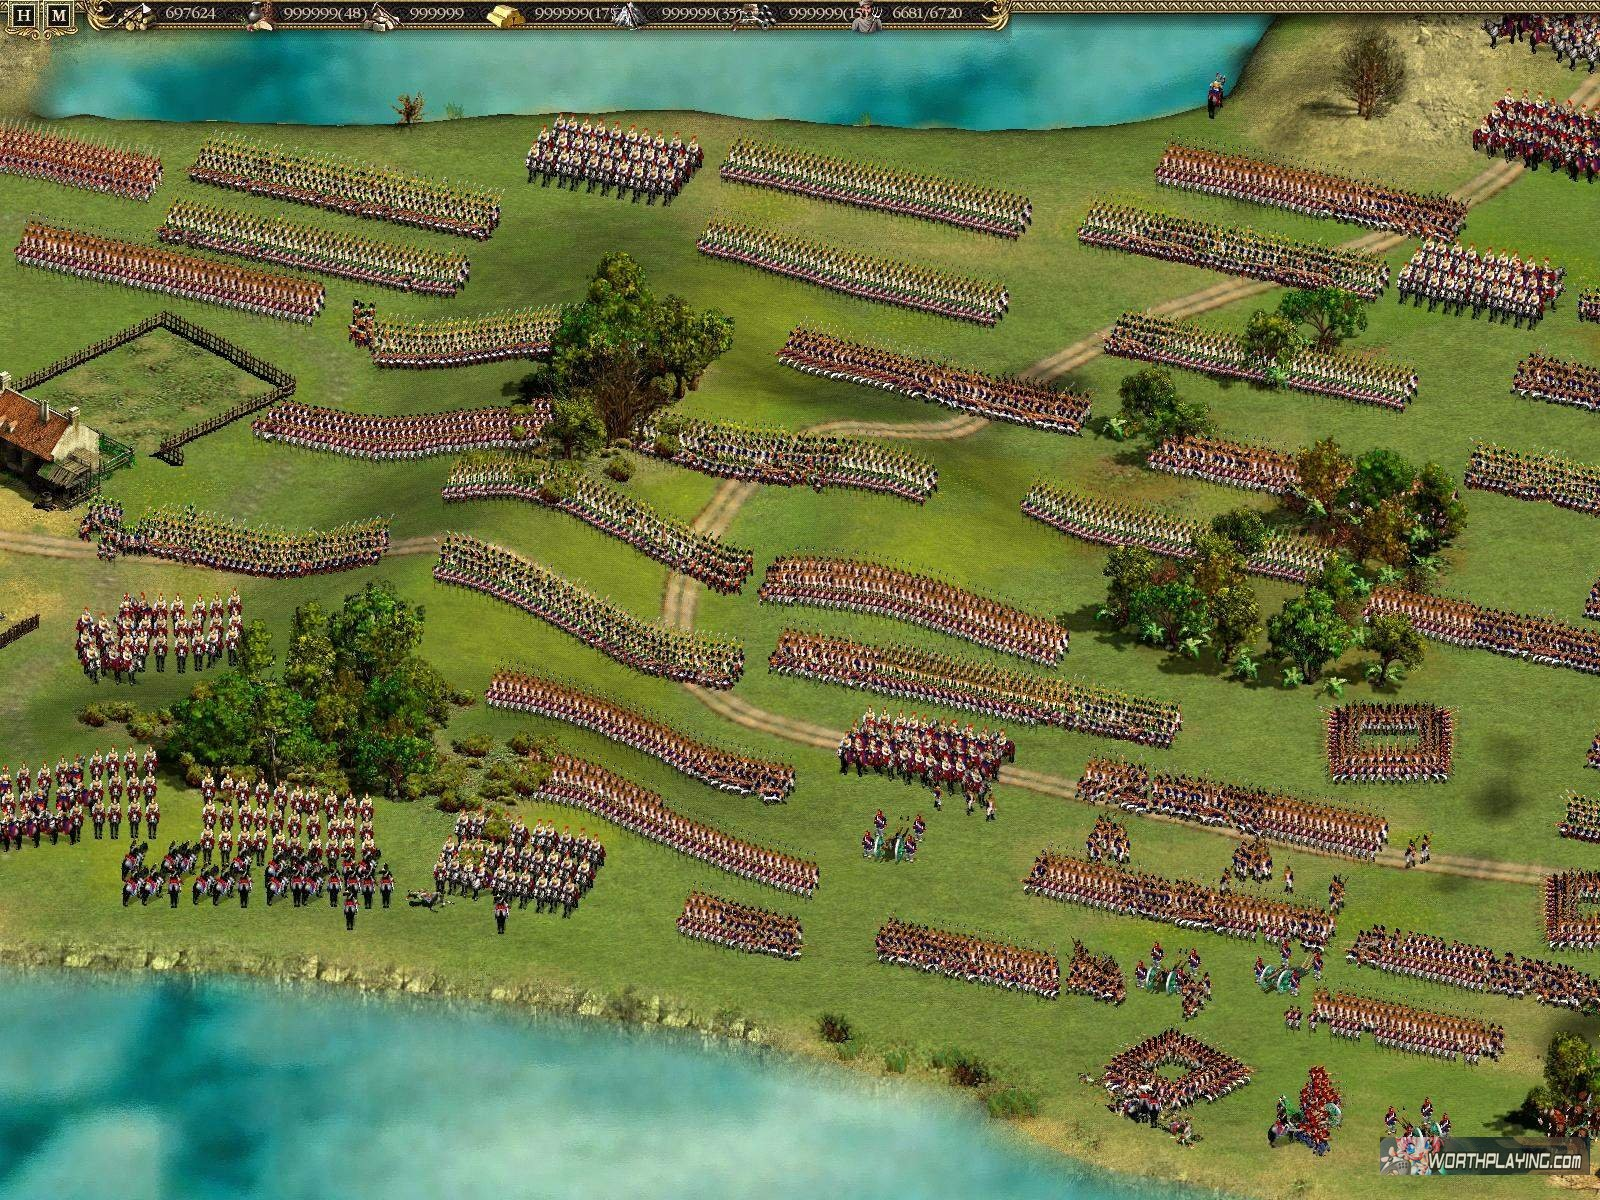
\includegraphics[width=\textwidth]{figures/cossacks2}
		\caption{Exemple d'une partie du RTS \emph{Cossacks~2: Napoleonic Wars}, avec de nombreuses unités, très proches les unes des autres. Au nombre et à la densité s'ajouteront, pendant la bataille, le mouvement, le désordre et le mélange avec des unités ennemies. Crédit : \emph{Worth Playing}.}
		\label{fig:cossacks2}
	\end{figure}
	
	\begin{figure}[ht]
		\centering
		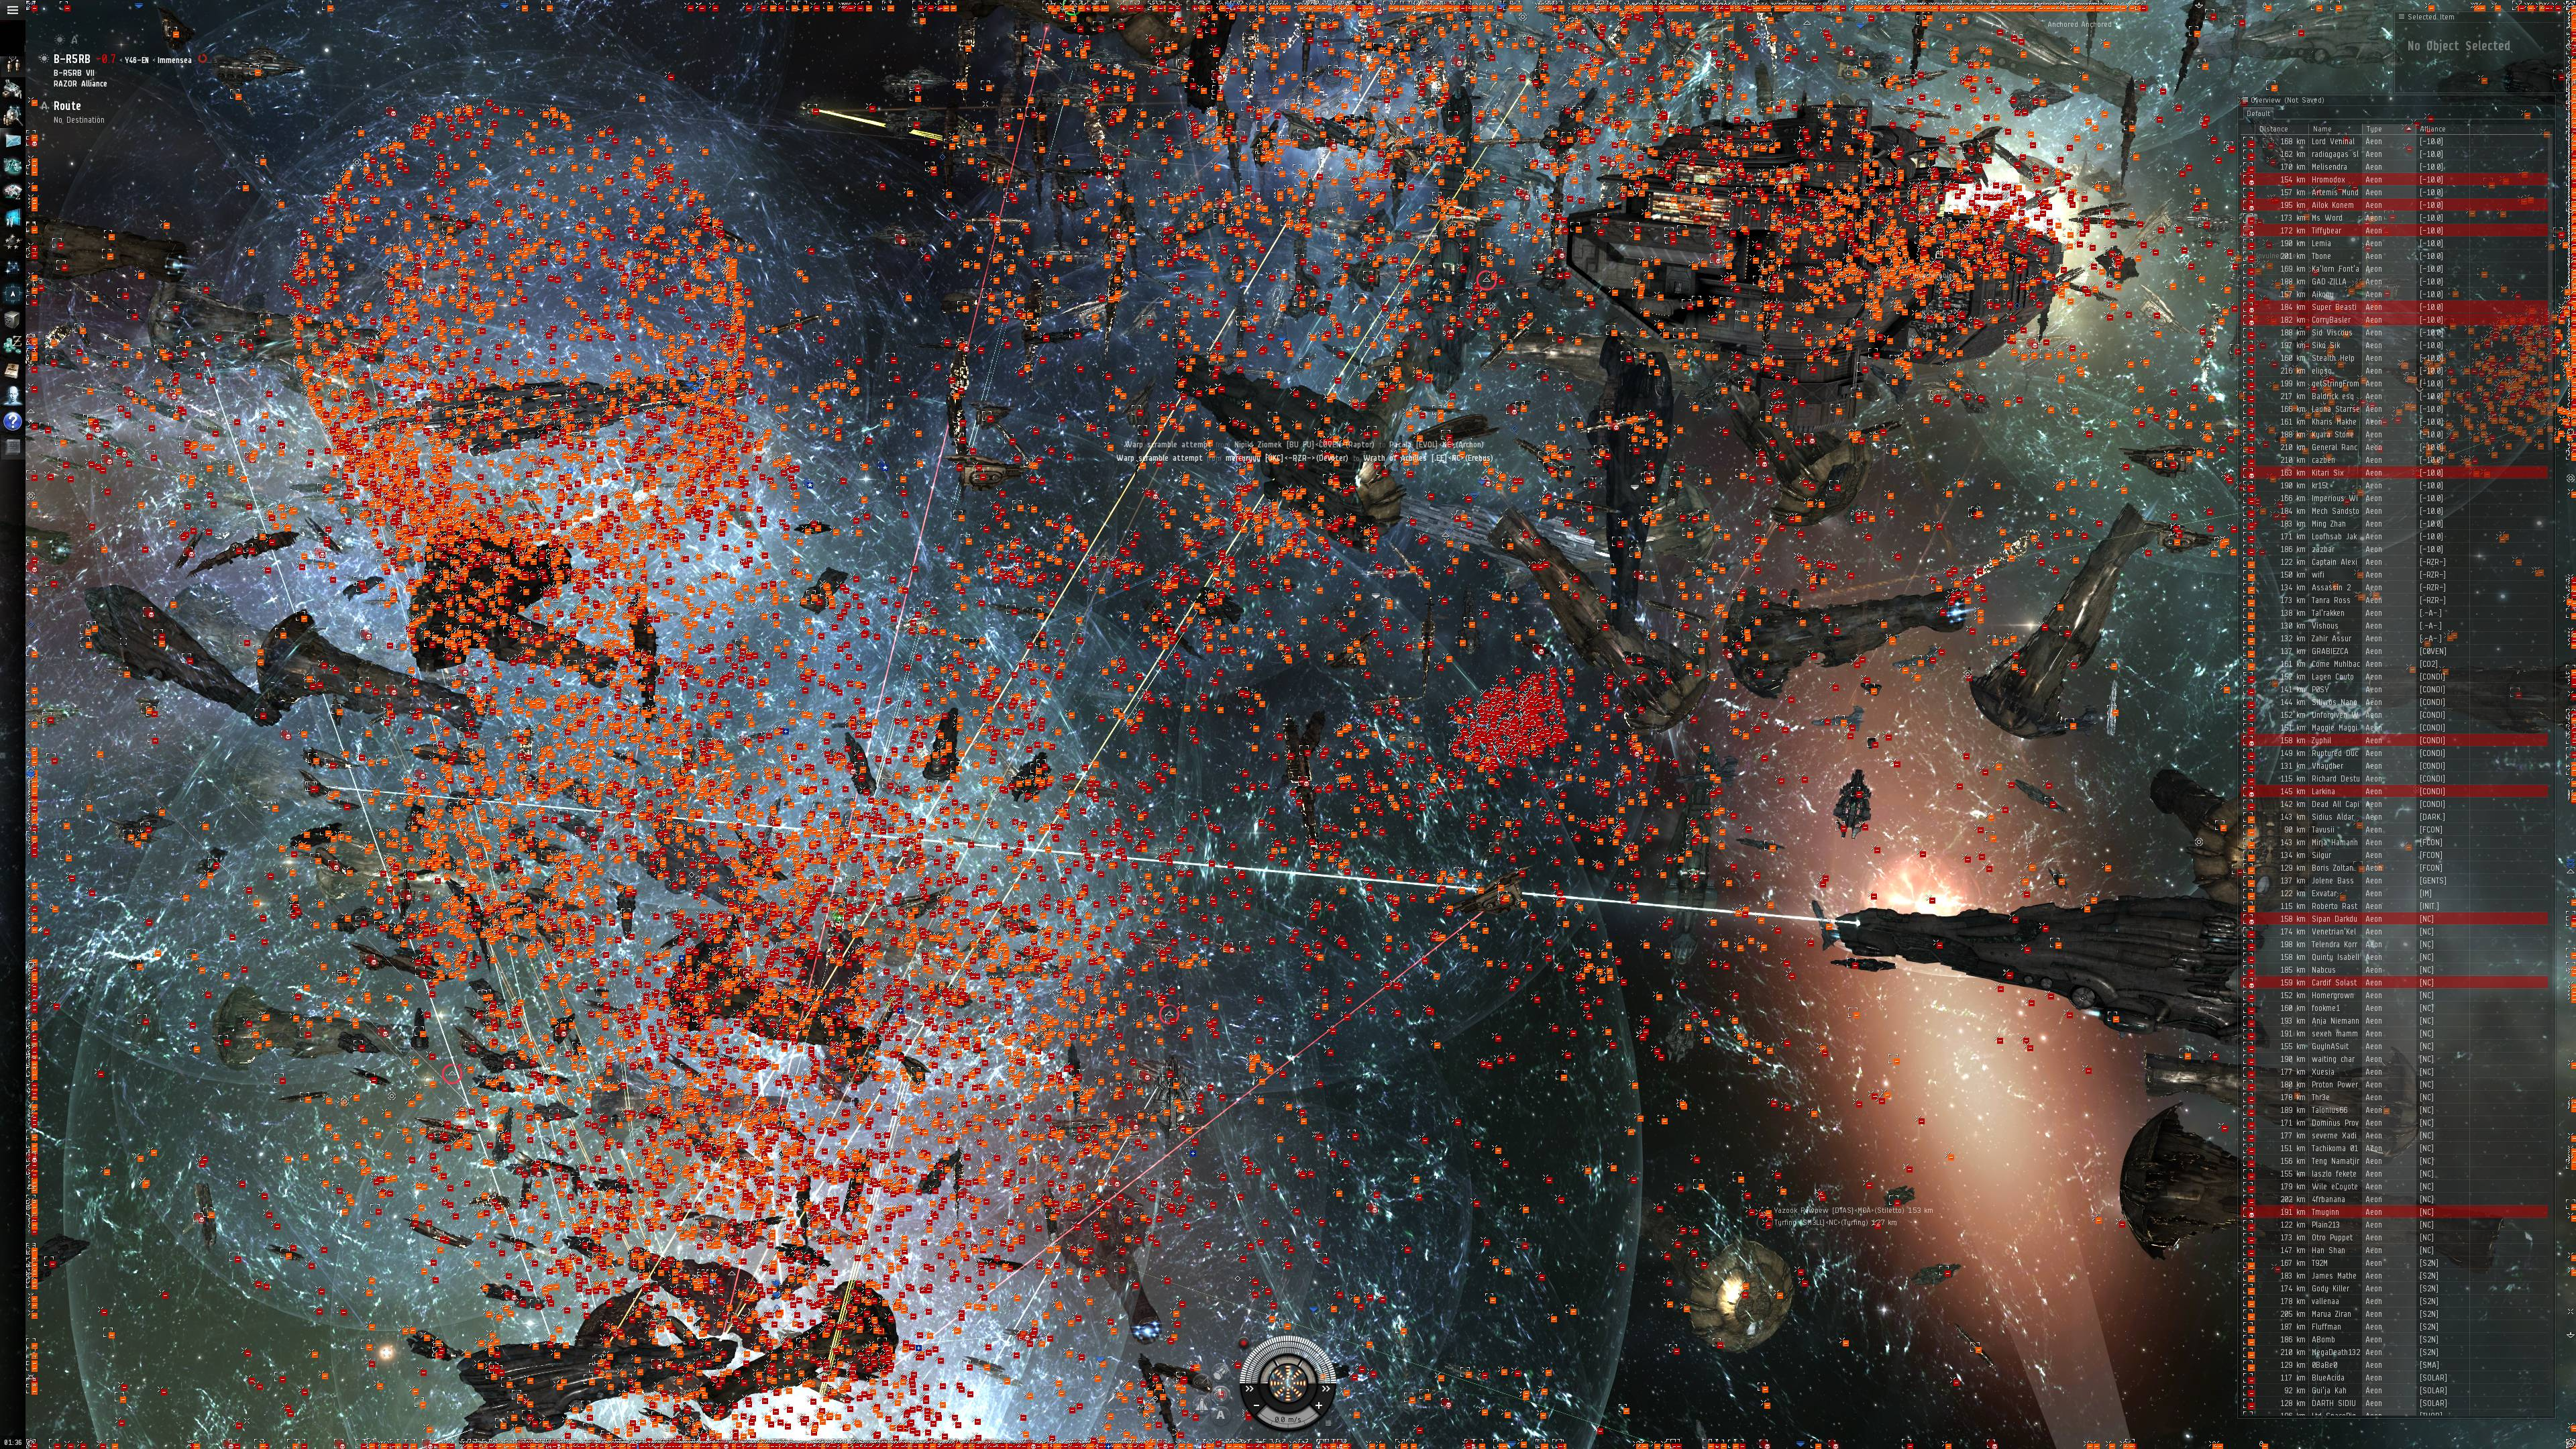
\includegraphics[width=\textwidth]{figures/eveonline}
		\caption{Énorme bataille dans le jeu \emph{EVE Online}. Le nombre précis d'unités est inconnu, mais chaque point rouge ou orange représente un vaisseau ou un drone, donc une cible potentielle. Au-delà du nombre extrêmement important de cibles, ce cas présente la difficulté d'être en trois dimensions, ce qui complique la saisie et implique un haut niveau d'occultation, en particulier pour les petits vaisseaux situés derrière un vaisseau capital ou de grande taille. Crédit : \emph{EVE Online Community}.}
		\label{fig:eveonline}
	\end{figure}
	

	\subsection{Arènes de bataille en ligne multijoueur (MOBA)}
	Les jeux de type MOBA sont caractérisés par un petit nombre de cibles (de l'ordre de quelques dizaines, tout au plus) rapides et imprévisibles.

	\paragraph{}
	Le \emph{wiki} du jeu \emph{DOTA~2} fournit des informations très précises sur les caractéristiques de mouvement des unités principales~\cite{dota2}.	 Celles-ci sont reproduites dans le tableau~\ref{tab:dotamoves}.
	
	\newcommand{\newrow}{\bigstrut[t] \\ \hline}
	\begin{table}[ht]
		\centering
		\begin{tabular}{ p{0.25\textwidth} c c }
		Héros				&	Temps de demi-tour (180°)	&	Vitesse (unités arbitraires)	\newrow
		Lifestealer		&	0.094 s				&	315						\newrow
		Shadow Fiend		&	0.094 s				&	315						\newrow
		Faceless Void		&	0.094 s				&	300						\newrow
		Batrider			&	0.094 s				&	290						\newrow
		Bristleback		&	0.094 s				&	290						\newrow
		Phoenix			&	0.094 s				&	285						\newrow
		Earthshaker		&	0.105 s				&	310						\newrow
		Magnus			&	0.118 s				&	315						\newrow
		Storm Spirit		&	0.118 s				&	285						\newrow
		Luna				&	0.157 s				&	335						\newrow
		Gyrocopter			&	0.157 s				&	315						\newrow
		Keeper of the Light	&	0.188 s				&	335						\newrow
		Pugna				&	0.188 s				&	330						\newrow
		Leshrac			&	0.188 s				&	325						\newrow
		Skywrath Mage		&	0.188 s				&	325						\newrow
		Lich				&	0.188 s				&	315						\newrow
		Outworld Devourer	&	0.188 s				&	315						\newrow
		Enchantress		&	0.236 s				&	335						\newrow
		Lone Druid			&	0.236 s				&	325						\bigstrut[t] \\
		\end{tabular}
		\caption{Caractéristiques de mouvement des personnages les plus vifs du MOBA \emph{Dota~2}.}
		\label{tab:dotamoves}
	\end{table}
	
	\begin{figure}[ht]
		\centering
		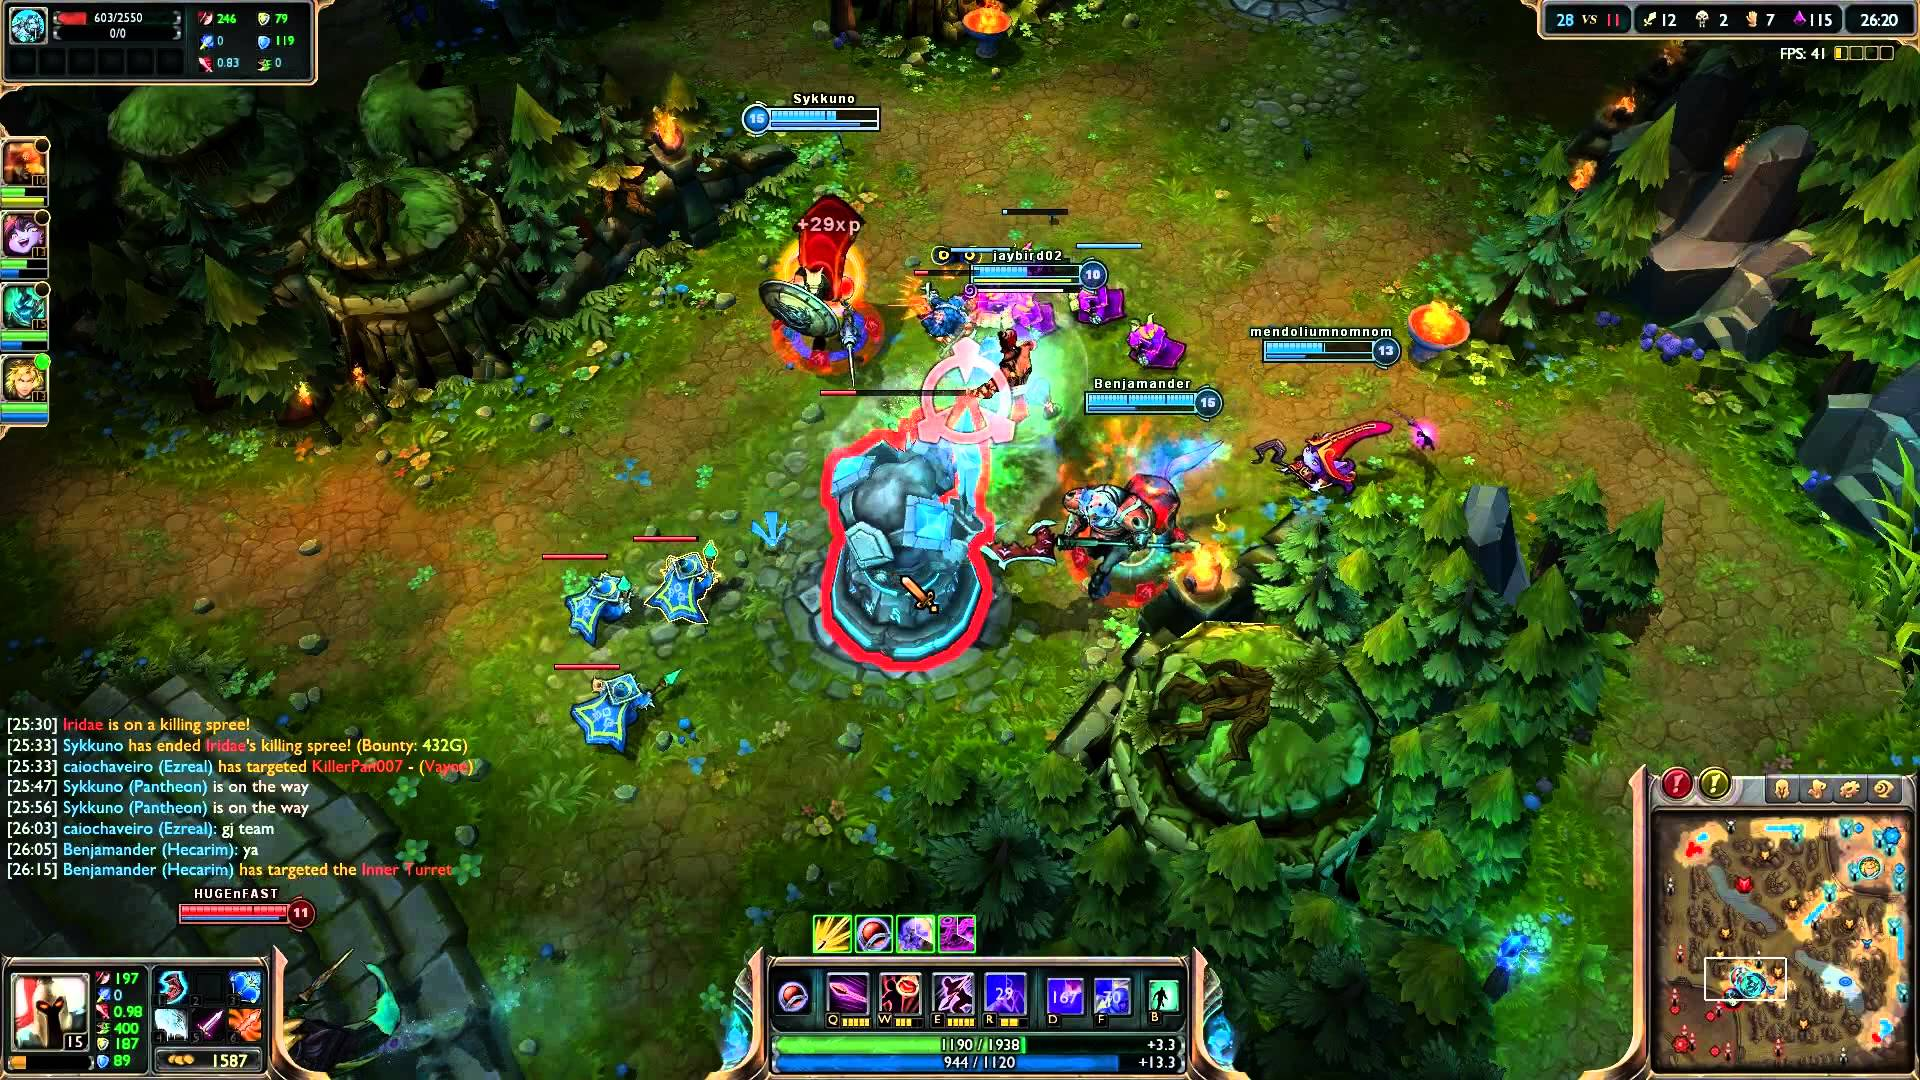
\includegraphics[width=\textwidth]{figures/lol2}
		\caption{Exemple d'une partie d'un MOBA, le jeu \emph{League of Legends~2}, avec quelques personnages. Crédit : \emph{Dota Geeks}.}
		\label{fig:lol2}
	\end{figure}
	
	\begin{figure}[ht]
		\centering
		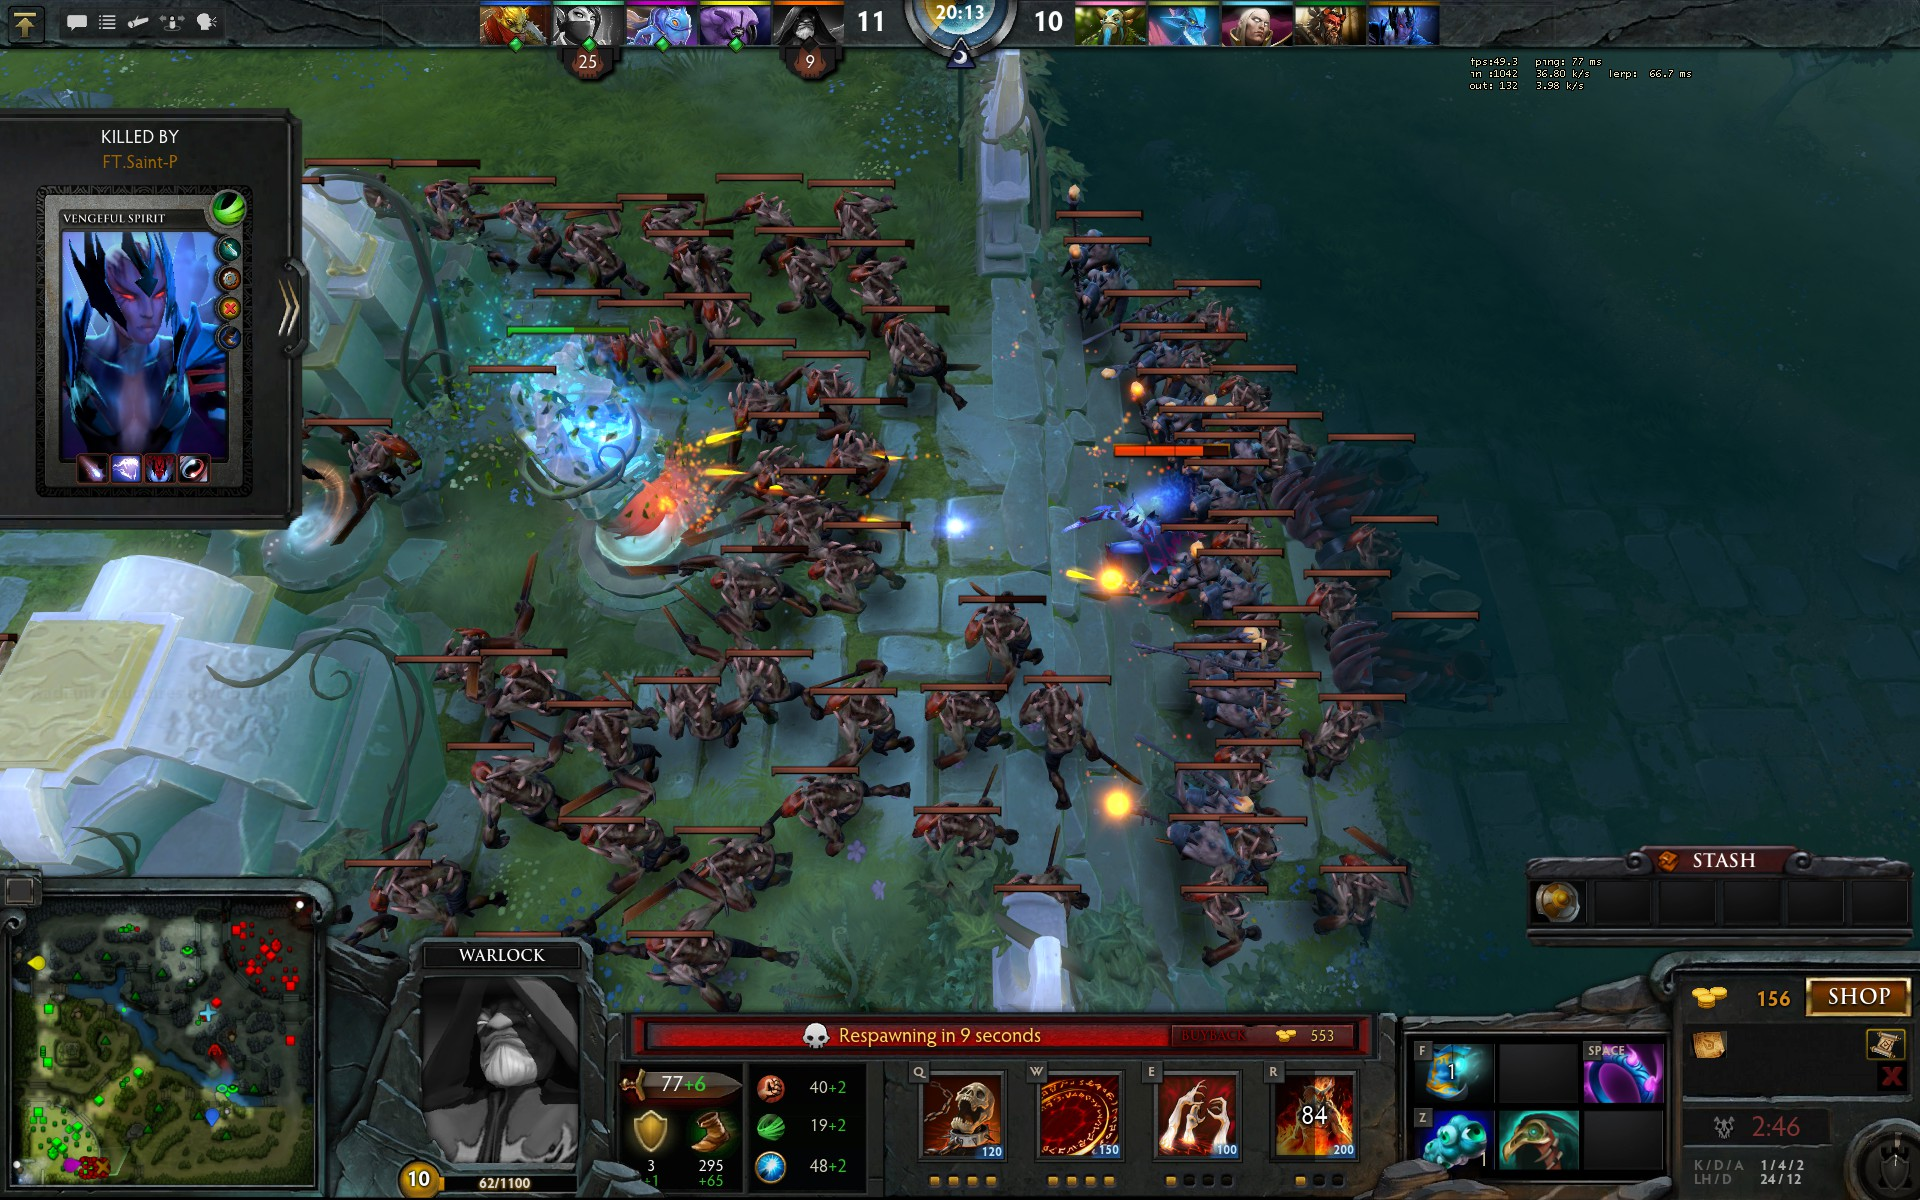
\includegraphics[width=\textwidth]{figures/dota2}
		\caption{Exemple d'une partie d'un MOBA, le jeu \emph{DOTA~2}. Les caractéristiques de ses personnages les plus vifs sont dans le tableau~\ref{tab:dotamoves}.}
		\label{fig:dota2}
	\end{figure}
	
	
	\section{}    
	Les tendances observées sur les cibles statiques demeurent, à savoir que la difficulté de la tâche augmente quand la distance entre la cible et le pointeur augmente, ou quand la taille de la cible diminue. Mais l'influence du mouvement de la cible empêche d'appliquer la loi de Fitts. Certes, la difficulté de la tâche augmente aussi avec la vitesse, [ref-mec-interact?] cependant, si la nature du mouvement a une importance cruciale, celle-ci demeure peu étudiée.
    
    
    
    
 The
difficulty of the selection increases while (1) target size decreases,
(2) target velocity increases and (3) target density increases. The
selection is even more difficult in 3D environments (filmed or synthetic
environments) because a target of interest can be occluded
by others targets. Selecting someone in crowds with a surveillance
video system is an example of a dense environment with small targets
and occlusion. In some cases, like in action sport footage, both
the objects of interest and the camera can move. Target movements
become unpredictable, and the selection is even more difficult.
In this context, as Hasan et al. [3] wrote, for completing the
selection ”the user must continually track the target and simultaneously
plan to move the cursor over it”. This underscores the key
point of the technique we propose here. Since the user follows the
target for selecting it, the Hook technique tracks the cursor behavior
for assisting the selection. Indeed, observing the history of cursor
displacements, and the history of distances between each target and
the cursor, the system can estimate which target is tracked, and then
propose a selection to the user who just has to validate it. In other
words, the user follows the target of interest, and the system will
know which target it is.
This paper presents the implementation of this technique, and
two experiments which investigate its performance. Hook has been
compared to the basic pointing (non assisted pointing), and to Bubble
cursor [2, 8], for the case of 3D object selection. The first evaluation
involves a desktop configuration, in which pointing is done
on a standard screen with a mouse. The second evaluation involves
an immersive configuration in which pointing is done with a 3dof
(degrees-of-freedom) device. Both evaluations highlight the bene-
fits of this new interaction technique for selecting moving targets in
a 3D environment. More than simply improving the pointing time,
Hook drastically decreases the error rate and allows pointing targets
in high density environments, with high velocity targets that are not
possible to capture with other techniques.


	
		

\clearpage
